% The Susan's Requiem master file, Normal (PDFTeX) Version.

% Very few changes should be needed here except title and author for instance. 
% Make note the table of contents (very bottom of this file)
% pulls in all the chapter files which is why this is the master file. It hides all % the technical mumbo jumbo from the actual writing too.

%	For pandoc compiles, open and compile using the Main-Pandoc.tex file.


% UNIVERSAL SETTINGS
% document structure

\documentclass[12pt,twoside,onecolumn,openright,extrafontsizes]{memoir}
\usepackage[utf8x]{inputenc}

% ebgaramond font package
\usepackage[cmintegrals,cmbraces]{newtxmath}
\usepackage{ebgaramond-maths}
\usepackage[T1]{fontenc}

% Predefined commands
\newcommand*\NewPage{\newpage\thispagestyle{empty}\mbox{}}

% Custom TTF fonts
\newcommand\theban[1]{{\usefont{T1}{theban}{m}{n} #1 }}
\newcommand\enochian[1]{{\usefont{T1}{enochian}{m}{n} #1 }}
\newcommand\terminal[1]{{\usefont{T1}{vt220}{m}{n} #1 }}
\newcommand\terminus[1]{{\usefont{T1}{terminus}{m}{n} #1 }}

% Text macros
\def\chichenitza*{Chich\'{e}n Itz\'{a}}

% PACKAGE DEFINITION
% typographical packages
\usepackage{microtype} % for micro-typographical adjustments
\usepackage{setspace} % for line spacing
\usepackage{lettrine} % for drop caps and awesome chapter beginnings
	\renewcommand{\LettrineTextFont}{\normalfont}
\usepackage[ttdefault=true]{AnonymousPro}
		\makeatletter
		\newcommand{\verbatimfontfamily}[1]{
			\def\verbatim@font{\fontfamily{#1}\selectfont\tiny}}
		\makeatother
				\verbatimfontfamily{AnonymousPro}
	
% \makeatletter
% \renewcommand\verbatim@font{\small\bfseries}
% \makeatletter



\usepackage{titlesec} % for manipulation of chapter titles

% for placeholder text
\usepackage{lipsum} % to generate Lorem Ipsum

% graphics package
\usepackage{wrapfig}
\usepackage{graphicx}
\graphicspath{Images/}
\newcommand{\parasep}{
	\begin{center} 
		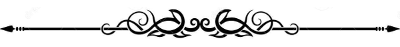
\includegraphics[scale=.5]{Images/hrule.png} 
	\end{center}}


% other
\usepackage{calc}
\usepackage{hologo}
\usepackage[hidelinks]{hyperref}
\usepackage{verbatim}
\usepackage{wallpaper}


% PHYSICAL DOCUMENT SETUP
% media settings
\setstocksize{8.5in}{5.675in}
\settrimmedsize{8.5in}{5.5in}{*}
\setbinding{0.175in}
\setlrmarginsandblock{0.611in}{1.222in}{*}
\setulmarginsandblock{0.722in}{1.545in}{*}
\setlength{\parindent}{0.5em}

% defining the title and the author
\title{Susan Rodriguez: The Quickening}
\author{Eric B. Teepell}
\newcommand{\press}{Susan's Requiem series prequel}

% custom second title page

\makeatletter
\newcommand*\halftitlepage{\begingroup % Misericords, T&H p 153
  \setlength\drop{0.1\textheight}
  \begin{center}
  \vspace*{\drop}
  \rule{\textwidth}{0in}\par
  {\Large\textsc\thetitle\par}
  \rule{\textwidth}{0in}\par
  \vfill
  \end{center}
\endgroup}
\makeatother
% custom title page

\thispagestyle{empty}
\makeatletter
\newlength\drop
\newcommand*\titleM{\begingroup % Misericords, T&H p 153
  \setlength\drop{0.15\textheight}
  \begin{center}
  \vspace*{\drop}
  \rule{\textwidth}{0in}\par
  {\HUGE\textsc\thetitle\par}
  \rule{\textwidth}{0in}\par
  {\Large\textit\theauthor\par}
  \vfill
  {\Large\scshape\press}
  \end{center}
\endgroup}
\makeatother

% chapter title manipulation
% padding with zero
\renewcommand*\thechapter{\ifnum\value{chapter}<10 0\fi\arabic{chapter}}
% chapter title display
\titleformat
{\chapter}
[display]
{\normalfont\scshape\huge}
{\HUGE\thechapter\centering}
{0pt}
{\vspace{18pt}\centering}[\vspace{42pt}]


% typographical settings for the body text
\setlength{\parskip}{0em}
\linespread{1.04}

% HEADER AND FOOTER MANIPULATION
  % for normal pages
  \nouppercaseheads
  \headsep = 0.16in
  \makepagestyle{mystyle} 
  \setlength{\headwidth}{\dimexpr\textwidth+\marginparsep+\marginparwidth\relax}
  \makerunningwidth{mystyle}{\headwidth}
  \makeevenhead{mystyle}{}{\textsf{\scriptsize\scshape\thetitle}}{}
  \makeoddhead{mystyle}{}{\textsf{\scriptsize\scshape\leftmark}}{}
  \makeevenfoot{mystyle}{}{\textsf{\scriptsize\thepage}}{}
  \makeoddfoot{mystyle}{}{\textsf{\scriptsize\thepage}}{}
  \makeatletter
  \makepsmarks{mystyle}{%
  \createmark{chapter}{left}{nonumber}{\@chapapp\ }{.\ }}
  \makeatother
  % for pages where chapters begin
  \makepagestyle{plain}
  \makerunningwidth{plain}{\headwidth}
  \makeevenfoot{plain}{}{}{}
  \makeoddfoot{plain}{}{}{}
  \pagestyle{mystyle}
% END HEADER AND FOOTER MANIPULATION

% table of contents customisation

\renewcommand\contentsname{\normalfont\scshape Contents}
\renewcommand\cftchapterfont{\normalfont}
\renewcommand{\cftchapterpagefont}{\normalfont}
\renewcommand{\printtoctitle}{\centering\Huge}

% layout check and fix
\checkandfixthelayout
\fixpdflayout

% BEGIN THE DOCUMENT
\begin{document}

\pagestyle{empty}
% the half title page
\ThisCenterWallPaper {1} {Images/Susan/woman-790590_960_720.png}
\halftitlepage
\cleardoublepage
% the title page
\titleM
\clearpage
% copyright page
\noindent{\small{This novel is entirely a work of fiction. The names, characters and incidents portrayed in it are the product of the author's imagination. Any resemblance to actual persons, living or dead, or events or localities is entirely coincidental.\par\vfill\noindent Pre-Draft Edition\space\today\\
		% ISBN\space\ISBN\\
		Source: https://eteepell.github.io/Susans-Requiem/\\
		\copyright\space\theauthor.   \par\vfill\noindent\theauthor\space asserts the moral right to be identified as the author of this work. This work is licensed under a Creative Commons Attribution-ShareAlike 4.0 International License.\par }}

\begin{center}
 	\centering
	
\includegraphics[width=0.25\linewidth=0.25]{license.png}
\end{center}

\newpage
{\tiny Disclaimer This deed highlights only some of the key features and terms of the actual license. It is not a license and has no legal value. You should carefully review all of the terms and conditions of the actual license before using the licensed material. You are free to: Share — copy and redistribute the material in any medium or format Adapt — remix, transform, and build upon the material
for any purpose, even commercially. The licensor cannot revoke these freedoms as long as you follow the license terms. Under the following terms: Attribution — You must give appropriate credit, provide a link to the license, and indicate if changes were made. You may do so in any reasonable manner, but not in any way that suggests the licensor endorses you or your use. ShareAlike — If you remix, transform, or build upon the material, you must distribute your contributions under the same license as the original. No additional restrictions — You may not apply legal terms or technological measures that legally restrict others from doing anything the license permits. Notices: You do not have to comply with the license for elements of the material in the public domain or where your use is permitted by an applicable exception or limitation. No warranties are given. The license may not give you all of the permissions necessary for your intended use. For example, other rights such as publicity, privacy, or moral rights may limit how you use the material.
}
\clearpage

% dedication
\begin{center}
\itshape
{
	\noindent
	{
		Nor shall this peace sleep with her; the bird of wonder dies, the maiden phoenix. Her ashes new create another heir, as great in admiration as herself. So shall she leave her blessedness to one. Heaven shall call her from this cloud of darkness; from the sacred ashes of her honour shall star-like rise as great in fame as she was, and so stand fix'd.\\
		\medskip
		
		\normalfont{William Shakespeare, Henry the eighth}
	}
}
\end{center}

%
%
%
%
% begin front matter
	\frontmatter
	\pagestyle{mystyle}
%%\chapter*{Dedications}
%{
%
%\section{Theme Song}
%	{
	%This book's theme song is David Bowie's ``Changes''
%	}
%
%\section{Dedication to Queen Lilith}
%	{
%
		%Bear with me here, \textit{Queen Lilith is the actual god and queen of vampires}. The real one, insofar as there could be.
		%	
		%I've done some research as I went along, what writer doesn't. I was creatively inspired to write about what happened to Susan on the alter of \chichenitza*. How she stood against the odds and will change the world for the better. The story of a hero who just happens to be a vampire physically. Somebody decent, with a dangerous side. I started it two or three months ago.
		%
		%I've avoided looking too much into vampire lore. The reason being I believed it would be horrible, mean and nasty. Either in the horror sense or in the campy sense.
		%
		%That isn't what I wanted to show in Susan. Neither maniacal nor glittery. I wanted to break the mold of vampire novels and \textit{not write a vampire novel.} I would write about an antihero trying to make a positive difference in the world without brooding a lot. That's gotten very annoying with other protagonists over the years. 
		%
		%I wanted to show strength, confidence, determination, responsibility, and someone protective and nurturing. A female hero that stands alone. A female hero that can be truly intimidating, and lay down some serious kick ass when it needs to be done. 
		%
		%\begin{wrapfigure}{R}{0.5\textwidth}
		%	\centering
		%	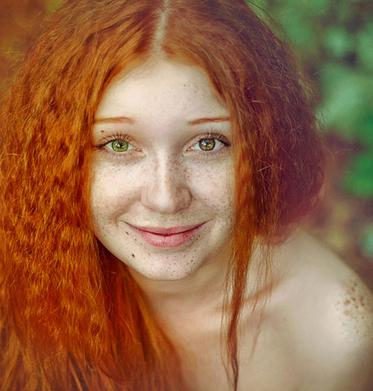
\includegraphics[width=0.50\textwidth]{Images/ginger-girl}
		%	\\ {\small Lilith, Queen of Night and Darkness.}
		%\end{wrapfigure}
		%
		%About a month ago or a little longer I had a rather forgettable experience in seeing a praying mantis under a case I had put down. I had never seen a praying mantis before that I can remember, I thought it was pretty cool. How it got there was a mystery there was nothing but concrete floor ten feet around me. I should think I would have seen it, but who knows. I felt bad for the little creature so I picked it up. It wrapped it's arms around my finger and squeezed, snuggling it's head against my finger. I thought that was very odd, but not having been around the creatures I presumed it was frightened and that's just what they did to stop from falling. I was honestly afraid it would bite me but it never did. I let it go into a bush to the side of the concrete platform.
		%
		%Something that day on a webpage had a passing mention of Lilith and Lamashtu. The mention of the praying mantis as the sacred animal grabbed my attention immediately. I read her biography in response. There was Lilith, so much like Susan as I had already written her.
		%
		%I'll write more on this amazing lady in an appendix after the story.
%	}
%}
	% \NewPage
\chapter*{Prologue}
{Not everyone is a Dresden Files fan so not everyone is going to know who Susan is or what she's been through. This series is going to be an independent endeavour from the Dresden Files proper so once her background is explained here it will be easier to get into the following story. She was very much a main character in the first three books, then disappeared until death masks skipping a book. There were six books before she had a major role in changes only to die at the end by Harry's own hand. Her hopes ended.\\

So here goes:\\

Susan and Harry met when she arranged an interview on the opening of his business as a professional wizard in Chicago. It was a couple years before the Storm Front novel. She was a reporter for the Midwest Arcane at the time which was a supernatural version of today's tabloid with stories like ``JFK’s Mutant Ghost Abducts Shapeshifting Girl Scout.'' Little did people know from time to time the stories were real! Susan even went into syndication.

She had a tendancy to hound Harry for a good story although she had an ulterior romantic motive, and made no attempt to hide it. Of course her romantic expression served her well in getting information as well.

She is attractive, intelligent, funny and appealing. Her motivations are clear and simple, and she is honest in pursuing them. She is absolutely relentless. She has used her sexuality in pursuit of information. She is very aggressive and was the one to ask Harry to dinner not him. Susan took Harry out for their first date and treated him. She has a smile all her own, a patent smirk with her lips quirking up at the corners. Her hair is midnight black. She has dark eyes and a deeply tan complexion.

The first three books were completely Susan. She could easily have been the other primary protagonist as far as I was concerned.

In Storm Front she asked Harry out for dinner. Well, kinda tricked him into dinner in a playful way. She wants what and who she wants and works hard to get it. She and Harry ran into a demon they needed to combat. A toad creature. They did it but barely, Harry called down lightning on it and Susan was vomiting most of the time from potions Harry had her drink. The date turned out to be the worst night of Susan's life. As well as the best story she had written so far.

In Fool Moon, the second book in the series, her appearances gained speed until about half way through the book she took the drivers seat. Literally. Getting Harry out of the mess he got himself in as well as being the driver for him and those he needed her to drive for. Including some young werewolves. Susan saved the day in this novel and Harry was along for the ride.

In Grave Peril Harry was about to marry Susan though it wasn't apparent until near the end. They are still dating heavily and very serious. She had her first sight of vampires in this book, but not her last. Harry got an invitation to a ball by a local vampire that just got promoted to the nobility. Susan forged an invitation to get in with Harry. Harry had protection under the accords but she didn't because she was never really invited. This particular vampire held him accountable for the deaths of two people she loved. Vampires being what they are in the Dresden series she swore to dedicate her life to exacting vengeance against Harry in one way or another. She found a perfect way. She knew about him and Susan so she stole Susan away and ``turned'' her. Basically this ended their relationship because Susan was walking a tight rope from that point on, she hungered but if she ever fed she would complete her change and become something else. No more Susan. For now, denying her hunger, she could survive and live as a human but arousal, exhaustion, or the smell of blood, or a number of other things might cause her to lose it and make a kill then game over.

That was the last we seen Susan, she did not have a part in the next novel but in the following one she did reappear briefly. She had been fighting the vampires in South America and doing humanitarian aid to the residents there. South America was the heart of the Red Court Vampire territory, the world pretty much ignores what happens there and it had gotten really bad down there. They followed a high ranking vampire back to Chicago (where the novels take place). She gathered her belongings from the city to take back home and intervened against the plans of the vampires while there. Harry and Susan got to fight again and went to a ball together. They even had a dance together. Then she left to rejoin the fight in Central and South America.

It was seven novels of wondering what happened to Susan and when she was going to find the cure for her vampirism. In that final novel ``Changes'' she fights with Harry to save the daughter they had together (that he didn't even know existed). In the end of the novel Susan makes that first kill and begins to change. Their daughter was saved from being killed in a sacrifice and Susan was killed in her place.

That is where the Dresden files story ends and the Susan's Requiem story begins. Her life will never be the same.
}
%
%
%
%
%


% table of contents
\clearpage
\tableofcontents*

% begin main matter
\mainmatter
\chapter{Susan Rising}

\begin{quote}
	``Martin,” I said, my voice low and very quiet. “Did you tell them about Maggie?”
	He closed his eyes, but his voice was steady. “Yes.”
\end{quote}

%using past tense
%scene goal
\lettrine[lines=2,lraise=0]{A}t that moment I was beyond saving. I've been on the edge ever since my daughter Maggie went missing, and now here we are at the altar of \chichenitza surrounded by vampires and their many minions determined to sacrifice my baby girl on the altar. I need to save her. 
%scene conflict
My emotions are on high, I've been far too close to losing it and now dumbass Martin tells me he led my only daughter to the slaughter. I couldn't see through my rage, I was so far beyond control I don't even think an immortal could have stopped me. My vampiric part foreseen it's victory over my will and poured it's power into me and drove me quickly and irreversibly to my kill. It shackled me to it's purpose and terror came from my soul to intermix with the rage. My humanity foreseen it's own death but was unable to pull back, the vampire in me had stolen control to ensure it takes the life it needs to fully emerge. Quick as lighting and lithe as a snake, I took Martin down hard and made the kill with complete abandon. 
%scene disaster
I knew what was going to happen to me but Martin was calling the shots, using the one thing that would be successful in causing me to lose it. To really really lose it. I just didn't care. I desperately wanted to care. I could do nothing but devour his life blood. I tore out his throat the feeding was so vicious. When he was dead I was changing. It was too late, I couldn't take it back. I had control of myself but only for a few moments. Oh my God the pain, horrible intimate euphoric pain. Searing with power and pleasure as I experience the wretched agony of my flesh tearing from the inside out. I started to feel the pain give way to a new mass, a new body not my own was devouring me and emerging in my place. The monster has been set loose in me, in my loss of control I sacrificed a life to the slumbering vampire and brought it forth to consume me. I think my hands came first as they were elongated and clawed, breaking through my skin. I seen the new being crawling beneath my skin like a snake or worm, a ghastly sight to behold.

She is coming, the vampire that I am to be, she is not me. I could feel the others coming, other vampires. I heard the memory of the Red Kings call to battle. I hear them, I feel them. My vampire half is becoming whole in me, while I live it now coexists with me but I will not be here long. My soul is soon to be consumed. Harry reminds me I am the youngest of the red court now, I can destroy them all by my sacrifice. I can take every last one of the red court. I scream to Harry to save our daughter Maggie. Maggie was all I could think about, I have to save Maggie.

Harry took Maggie from the altar as gently as he could, and laid me down. I am still being consumed, I haven't much longer for my humanity to live. Harry promised me Maggie will be safe, I felt confident in his words. That didn't completely absolve my worry, and it did nothing to absolve the sheer terror I felt over what is happening to me. Harry was going to sacrifice me. I've never been so scared in my life but I still knew it would preserve me from the completion of my transition, and destroy the monsters that have caused so much suffering. Oh I was so scared. He closed my eyes with his hand, and kissed me. It was a sharing of our blood and our tears. I cried out to Maggie, perhaps just to tell her everything will be ok, but I don't think it came out as more than a whisper.\\
%no, and furthermore

\textit{Then Harry cut my throat, and I was dying.}\\

All was black, but for less than a moment. Lighting came down from the heavens and struck me in the darkness, maybe it was a dream, but it kept frying me for what seems like forever. I felt the consumption of my body, well, come to completion. Bye bye human me. After a time I felt myself floating up and seen myself, my blood flowing out from all over the altar. My body glowing and sparking with energy repeatedly, like when lightning hits a large transformer in the street. The energy slowly being absorbed. The vampires were gone, my friends survived. I am dead. The whole red court is gone including myself the youngest of their kind. Thank God for that. Soon enough I know that sweet chariot is going to swing low and come to carry me home.

Harry was in such pain. I could see it. I rested my hand on his shoulder and tried to talk to him. He neither felt it nor heard it but I could do no less. Harry is standing there, in shock, not moving. The vampires all fell leaving nothing but black sludge. The infected were mostly killed except the younger ones, since the vampire part was killed and it was what was keeping many young, even alive. 

%scene continued with Erlking
Walking toward the altar is the Erlking and I take my place beside Harry.\\

	``Huntress, Sir knight, well met.''

I had to check but yes, I'm still a ghost. I turn to Harry with a tear. Yes ghosts have tears, apparently.

``To you as well.'' I said.
	
	``I hope thou wilt be pleased with the strength of thine new nature huntress. Nay, I played no small part in bringing it to you. I was most certainly pleased that thou wert the first to have been my guest. Thou art honorable and wise my dear, such cannot be hidden in you. Thou likely thinkest that thine visit to mine realm twas coincidence? Be not a fool I willed it so. I was needful that you could be near me, that I might know that thou wert pureborne.''

	The Erlking smashed Maggies shackles and placed her in Harry's hands. ``Thou art the greatest hunter of thine kind, I cleared thine path for you. I ensured that thou wert slain. Your life has been hideous child, thou wert pitted against thyself like thou wert thine own prey, to live thou wouldst needfully refrain from the kill and blaspheme thine own nature. It is now abolished in you. May you and yours now hunt in freedom and rejoice in the kill. Thou hast redeemed thine species in the shedding of thine own blood. Thou art now free to join your hunt without fear of destruction. Thou canst replace these dishonourable wretches with thine own children as thee see fit. A pity I could not get the chance to hunt the red king and his ilk myself.''
	
	I don't see where I can enjoy the hunt as a spook, or how me and Harry can make little spooks together. Bloody Markov chains I'm gonna have to wait out the answer.

``Perhaps you might elaborate more and explain what you mean?'', I said.
	
	``Thou art always welcome as mine guest o' queen, then shall we speak together by the fire enjoying our kill.'' The Erlking bows low to me. He looks at Harry with a sort of piteous eye, ``I promise that by my hand thine mate shall not be slain. I know thine mate twas torn from thee in a most hideous way.''\\

Then at that he swiftly left on his way. Harry seemed to come to his senses after what seemed like forever. Just as well he would have been confused as fuck. I know I am.  As a matter of fact a helicopter came in and landed taking in a couple people, then left. Harry still stood there with a thousand mile stare, holding Maggie. I stayed with him, I wouldn't leave him, even if he couldn't see me. I hear our friends conversations with my enhanced hearing. I sat there with Ebenezer and Harry while they chatted, they were none the wiser. It's amazing he is actually Harry's grandpa, I wonder what other wizards are in Harry's line. I wonder if my Maggie will be a wizard when she grows up? I'm not sure how to feel about that. I still sat there with Harry as Karrin came over to chat. Harry was determined he was going to give up Maggie for adoption. Oh my God I was scared, but then I realized what I did but giving her up to a familiar family was pretty close. I hope he decides against it but if he does let her go for a better life I would understand. The rest escaped into a portal and Harry's Faerie Godmother remained. I felt my purpose accomplished and as I heard the sound of a vehicle approaching I begun to feel light and being pulled somewhere. Well this is it then, I'm going home to the family I've never known. I get to see the hereafter and Godwilling enter into paradise. I was being pulled toward the altar. My body was melting into the same black sludge as all the reds had, mingling with my blood and seemingly seeping into the stone of the altar. As it did I was drawn into it rather than being released like I expected. I was terrified that my soul was meant to be trapped in \chichenitza forever.\\

Fuck.\\

Then I was sucked into the alter.\\

I guess that chariot isn't swinging low for me after all.\\

%scene disaster
As I lay there some words I heard earlier that day keep repeating in my mind.
\begin{quotation}
	``You son of a bitch,'' I said, ``You fucking traitor.''
	
	Martin’s expression flickered at my words. But his eyes never left the Red King.``I give you the Fellowship of St. Giles, my lord,'' he said. ``And I beg you to grant me my reward.''
	
	``Reward,'' I said, blind with rage,``What could they possibly give you, Martin, to make it worth what you’ve done\dots''

	``And what do you get?'' I said to Martin.
	The Red King states, ``Ascension.''
\end{quotation}

I hear him say ascension over and over again in my head. What is happening? 

%transition 4days
I did lie in the alter many days. My eyes could see the sun rise and set upon that altar, the surface of my solid tomb. I could feel the warm sun and hear the breeze and chattering tourists. I thought to myself that it's not so bad being stuck here. I have company, I'll get used to it.
%sequel emotion

I'm dead. The silence of this altar allowed reality to catch up with me. My life has been wasted. Ever since I was half turned life has been nothing but a struggle and getting killed has been my only release from it. I knew it would be that way though, deep in my heart I knew the only escape was death. The fellowship had been working on a cure for a vampires turning ever since the fellowship came to be hundreds of years ago. They never found it. Either I must die, or make a kill and allow the vampire part to consume me and take over. I think Harry is going to be ruined, the man is going to need full time therapy when he gets back. Sure he's tough but this is too much. On top of that if Maggie were aware of anything going on she will be scarred for life. I want to just hide in this altar indefinately, just hide away from the reality of what happened outside of here in that world outside. Hide from the hereafter and from what other transitioned souls might say in my afterlife. What am I really? Innocent or guilty of making a kill? Depends on who you ask I guess. I place no blame on Harry I climbed right up on the altar and waited on him. The question is am I culpable of something?

What an odd word to use when Martin would perhaps be promoted within the court, raised to an office of a position, ascension is like to a king ascending to a throne of Christ ascending to heaven or a lesser being ascending to Godhood. Would the Red King really want Martin, being of a traitorous nature, to take power to himself in a worldly way much less a supernatural way? Really, who is Martin to raise him up to any position when any given responsibility would be poorly invested in anyone who could have executed such a grievious betrayal as he had done. The red king is mad but I don't see how he could be that mad. So if it was intentional it may be something the king was going to inflict him with, ascended and enslaved. Given significant power. Or something Martin was to cause, his actions are to cause and ascension of something or someone else. Everything is speculation right now.
%decision
I need to find out, something big is going on I feel it. I need to understand it and what role I'm playing in this game. who is the mastermind and what are his intentions? I'm in danger even as a ghost. Since I got sucked into this altar it's pretty clear to me something is weird and why would the Erlking have said that weirdness that he did? I'm all questions and no answers, very fews clues either. I need clues. I need answers.

%action
It's midnight, on the fifth day. I feel my body rise, the next thing I know I'm lying on my back on top of the altar. My arms are crossed fists on shoulders, my head laying to the side. It made me think of a song, ``walk like an egyptian''.

\parasep
%switch now to present tense, flashback is concluded.
%scene goal

I look at myself and shudder.\\

Oh God, I'm not human. This is the true form of the red court vampire. I really did complete my change. I feel normal though. I seem to be physically a typical red court vampire except maybe the odd thing, like talons rather than claws that resemble razor sharp scythes. I'm hungry. I'm very hungry. Oh my God sweet Jesus mercy and pass me an artery hungry. I have control for now. I catch the scent of human on the breeze and crouched low in a tiger's purr. The sound catches me by surprise as the red court never made such cat sounds that I'm aware of. I'm a little different somehow. I concentrate a little while and manage to put on a flesh mask, a convincing one, but being naked I decide to forego the flesh mask and go with the xenomorph look. A xenomorph born of a man sized vampire bat host is the essence of what a red court vampire true form looks like. H. R. Giger never goes out of style. 

All around, throughout the countryside, it sounds like popcorn. Anarchy has descended in the land and armed conflict is everywhere. People and paranormals are struggling in the power vacuum and damage caused by the destruction of the red court. No good deed goes unpunished.
%scene goal

So here's what I need to do then, find the nearest town and investigate more of what happened. I would look around here but I'm hungry. I've held my hunger as an infected I should be fine now, but not for long. Maybe I could take a couple sips while I'm there, I'm not that bad off right? A little nibble, that's all.

%introduction conflict, hunger drives her into damian, who prevents her from getting further

I leapt to the edge of the temple, onto the stairs of the pyramid. I'm smelling the air, I can't help it, my vision goes from black of midnight to the shadows of twilight as my eyes see through the darkness. I smell life-blood and I see the glow of human life off in one direction, at line of sight. With a growl I'm off. A growl, like a great cat. Not a shriek, wail or hiss as would be expected of my kind. Heh, my kind. Shoot me now. I laid tracks fast for the source of the radiance and I see someone driving a truck down the road and I hit the windshield at a speed faster than the truck was moving and smashed the bloody carcass out through the back window onto the road. I utterly destroyed the man tearing flesh from limb with my claws, chewing, sucking, lapping and gulping every last bit of the poor victim. They wont even be able to identify him with dental records. I'm too hungry to have any control. I genuinely hope someone just shoots me.

A black court vampire appears. He seems to be quite unusual, like from the Sherlock Holmes era, except for the chainmail gambeson draped over him and the combat boots he wears a very upper class Edwardian suit. God he looks cold as ice even for a vampire. He throws down a child he just consumed, a little 4 year old boy, blonde hair and freckles. dead and gone. He pops his collapsible top hat, and bows to me with a flourish of his hat. Then fills a pipe and speaks.

``Has anyone ever told you of natural selection? Foolish morsel decided upon himself to go forth into the night and deep forest I know not why. Most certainly I can say of him that he quite simply is a feeble-minded child. It is well that I had found him that he might be most effectatiously culled from the local herd. Alas it nearly came to pass that the noble vampire society might have been deprived of this most delicious morsel should he have perished in and of himself. Do you not agree dear lady? Yet as you are a most grievous poacher, oh what shall I do?''

``You fucking monster!''

``Ah yes, this I have heard many a time. 'Tis rare though that I should hear it from a kindred species, 'twould seem like to the pot calling the kettle black as they say. Let it be agreed then that I am a monster. So what of you dear? I cannot accuse you of wasting a single drop of that kill all chopped up and wrung dry so don't you dare be hypocritical. At least my kill is in one piece. I'm proud of who and what I am. Are you? I don't think you are.''
% scene climaxing

At that he withdraws something from his gambeson, damn. He's got a jar. Like as in ``A Jar'' trademark pending, a weapon I'm sure was first devised by the fellowship against the red court. Although not really used for anything but vampires, they may work on other supernatural entities or powers. They have no effect on humans. On vampires we used them as grenades and mines, hard as hell to get them triggered but when they do it's a guaranteed capture and the vampire is trapped in the jar which acts as a spirit container. We would then bury it deep, if we could drop it down with a post-hole digger we would. That way, just as Damian said, the creature would sit and rot until the second coming.

Problem is, now the shoe is on the other foot. I have no idea how he could be so confident that he won't get trapped but being I'm of the vulnerable species now I'm in hot water. He must be either crazy or stupid. My money is on crazy.

He casually taps the pipe empty on his gambeson and replaces it in his pocket, then drops his walking stick aside. He holds up his right hand and with a few words a slow moving black and purple ball slowly forms in his palm, the size of a basketball. I understood the words though I shouldn't have. I've never known such a language.

He said, ``Livyatan niis d ol nobloh tzrvt ollor adin zerimah''

Instinctively I know it means, ``Leviathan come, into my hand forms a gentle flow.'' Although I have no idea of the implications of the words. I repeat the words in english out of curiosity and see black and purple mist, unfocused energy flowing around me.

He said, ``Most singular indeed you are. It was best that I should have the jar.''

Without much warning he said, ``Lhtchl'' and the ball hurtles at me, I throw myself and roll. The ball curves toward me, I vault behind a tree and the ball crashes into the tree. The tree makes a low moan like it was being subjected to an immense weight then is still. Even the leaves flutter far too slowly given the force of the wind today.

Then he said, ``Flereus niis lishloach mad setani prg lehashlich forth, pon in oyev'' and a ball of flame hurtled from his hand directly at me. Fire is not good, I'm particularily vulnerable to it.

To my surprise it burnt straight through that same tree and it fell to the earth. Of course it caught me off guard and I hurled myself just in time, it hit my left bicep burning it off straight to the bone and I wailed, the shoulder on my other side hit a rock hard on the ground where I fell and I wailed again. I leapt backwards with a shriek and came up to stand with two useless arms. I'm in big trouble now.

He decides it's a good time for a tackle, he leaps and I dodge, he lands where I was just a split second ago.

No he predicted it. His walking stick is special I see, he wielded it as a sword stick and sliced open my belly. I figured I was done for but the wound stuck and I managed to bear through the pain and land a hard kick on him. I break his neck, which heals itself before he falls to the ground. I really hate vampires. Myself included.

He grabs for the jar but I'm already on the road ready to speed away. he throws the swordcane hard and in crunches into my hip. I sorely miss my firearms. I had an automatic pistol once I really loved. Snap out of it Susan, don't drop now, fight.

I'm on the ground. I can't move. He is throwing the jar for the final attack. I'm at the rear quarter of the truck. My arms are working again. I throw a rebar off the truck which goes right through his side but it only redirects the jar slightly from my head to the steel quarter panel where it triggers.

It was right where it needed to be. Right in the sweet spot. Inky black smoke licked out of the jar and just as I was afraid of it enveloped me. It felt like being on the scariest rollercoaster ever. I shrieked. After that, I was a jar. It is surprisingly spacious for a vampire in a jar. I never knew that. Rather than infinitely small it's infinately spacious. Must have something to do with the magic used. A rebar sails into the truck and it starts to roll backward crushing the jar. I'm released seemingly with a pop to land on the road with a plop. My body feels like jello and I yank myself to my feet by grabbing the truck and hurling myself to the other side.

I hear a familiar word of power, damian says, ``Fuego'' and a laser beam of fire pierces the body of the truck and wings me on the way to the ground on the other side. I howl and wonder what can I possibly do to overcome someone proficient in magic. I tear off the back quarter panel and narrowly block a rebar yet it still shreds through and narrowly missed my right arm on the way down. Split in two I swung the one side of the quarter panel at him knocking him to the ground and head to the side of the road. An unfocused ball of fire burns toward me and I turn what's left of the quarter panel and deflect it skyward. the impact sears my hands as the metal turns molten and throws me into the treeline. I break into a run deeper into the treeline and hear an animal behind me. It closes on me as I run then it's jaws tear at my ankles. I fall. Damian appears ahead of me and I roll as he hits the earth with his fist and around me the earth begins to buckle and split. It splits deep and my hands grasp the other side of the fissure to catch myself from falling in but it is still spitting and soon I won't be able to reach the other side.

Damian says, ``Wonderful my lady, 'tis most suitable that you should perish for all the trouble you seem to cause me. I do forsake the chance of casting you into the jar you are hardly the willing maiden with such a spectacle you have displayed.''
% scene disaster

I fall into the crevase, grabbing into the rock face and landing on a small outcropping on the way down. Holding onto a couple awkward handholds my feet are hardly wide enough to span the size of the outcropping. Soon I'll be heading into the lava pool at the bottom with the shaking of the ground as the ground continues to split.

Damian says, ``Well adieu then dear lady, may I suggest that you should refrain from holding onto false hope and embrace the fires below. I assure you your destruction will be quick then there shall be no more pain nor suffering of this most noble vampire existance. I wish you could have embraced your nature and come to be my comrade and not mine enemy.''

At which point he heartlessly walks away. I expected such heartless behaviour of course from a creature who could make a kill of an innocent child. I have a rather perplexing situation now though, I can't reach the top I'm too far down. Another quake causes part of the face of the cliff to fall and I grab new handholds just in time as the old ones give way. I'm leaning farther and farther over though I'm going over. I pull hard on the handholds and manage to get myself back against the rock face. Oh God what the hell is going to get me out of this. I look around but only see sheer rock face with handholds I cannot reach. Another quake causes more erosion of the cliff face. I try using my talons but it just erodes the rock face faster rather than grabbing hold. Too much earth mixed into the rock. Another quake and the outcropping I'm standing on falls. I'm holding desperately onto the handholds and I scream this is freaking crazy I'm going to die right here. No matter how much I can regenerate a lava pool is permanent. A handhold crumbles then another quake causes the other to crumble and I'm in freefall. I slash my talons into the rock face and manage to slow my descent but there is no other outcropping to save me. The lava pool is getting closer then my talons hit something substantial, solid rock, the impact jars me and my feet don't seem to feel the rock face anymore. It seems to be some sort of tunnel. Oh thank you Odin. I rock my body like a pendulum and throw myself into the tunnel. This is something that looks untouched by man, stalactites and stalagmites, dust on the floor of the tunnel undisturbed by any creature.

I fall on my ass, shaking with adrenaline. OK I just need to figure out how to get back up the fissure. What's around here. Is there at least some vine? The ground rumbles again. I look out into the ravine and see the walls closing back together. Oh man I gotta find something. My heart is in my throat, I'm scrambling around in the pitch darkness with vampiric vision to find something to get me out of here and back to the surface. Nothing. Absolutely nothing. Another rumble. I grab a stalactite and place it between the two 
%disaster, and furthermore
walls. Another rumble, the stalactite shatters. The walls are sealed. My fate is sealed.

I can see in here with vampire vision. The tunnel is wide open. A room essentially. No way out.

%sequel, emotion
I sit down on the floor of the room. Now what. There must have been something I could have done to stop this. Harry would have found a way. He gets in this sort of thing all the time. This really isn't my bag. Clandestine strikes. In and out. Fellowship style. I can do that. I have no right to be in a battle with an entity like Damian. I was outclassed. I should have ran, found a way to hide. Just let him jar me maybe someone would find me. What if he buried me though? Noone would ever find me. What was I to do? Now I die here. Maybe this is going to be my jar. I'll just go crazy in bloodlust and fade away. Hidden beneath the earth, noone will find me and I can harm noone. He was right, I should have saved myself the pain and just thrown myself into the lava pool. I want to die anyway. I don't want to live as a monster. I don't want to be this creature. Why do I feel this way though? I've never known a vampire to display such self loathing. They are narcissistic, maybe even psychopathic. What am I? I am so terrified. I want to die but I don't. I want to live. Somehow. To find a cure, to refrain from the feeding somehow. To stop killing. To stop hunting. Should I even attempt to find a way out of this. It's futile. Why should I?

%sequel thought
To stop the vampires that's why. To find a way to defend people against the supernatural forces. I am the only one with the strength of a vampire, the speed, the invulnerability against their hunger. They can't feed on me, we're made of the same stuff. I represent a hope for mankind. Despite being a human predator. Is that what they call an anti-hero? I guess that's me.

%sequel decision
Right then, time to get the frick out of here. I need to feed and I need to get somewhere to find out what happened to me. I have a purpose. I'm like the only vampire with a human soul. I don't know how but I'm important, I don't know how but I came to be for a reason. Some mysterious reason. I need to learn my purpose and fulfil it. I need to get out and back to the road.

%sequel action
I look along the walls of the room to see if there is a break into a further tunnel or chamber. In the twilight sight of my vampiric eyes I look as deep as I can but see nothing. On the floor of the chamber is nothing. Some dust but no footprints. Every once in a while I trip on something I should know is there. I look and see nothing. I must be exhausted. I lay down for a few minutes. What am I missing? Please don't tell me I was meant to die in some cavern. I was never a big cave explorer, although I can see how beautiful it is in these deep places.

I feel bad for messing it up. Walking all around scuffing up the floor of the cave and leaving it disturbed somehow. Like it's unclean in a way, having been touched by a person it's like it lost it's virginity leaving footprints all around. Hey wait a minute, I didn't leave footprints? Such a fine dust on the floor I should have left footprints. Something isn't right in this place. I swipe the floor with my hand, I don't feel dust. I look at where the rock face was and I see there once was a tunnel. The spell closed it off though. OK there once was a way out. Now there isn't. To hell with it I'm laying down, this is making me tired.

As I lay down I see on the ceiling what looks like a switch. A silver switch embedded in a green jewel. I think I get it. Tripping on things not here. Not leaving footprints. Some kind a veil. It has to be. I feel around the walls and find many indescrepencies, and something in particular I was looking for. I find what looks like a ramp along the wall. The creator of the veil would have been able to see though it and climb to the switch to disable the veil so others could see. I blindly climb up the ramp and sure enough it takes me to the switch. I move it over and the veil disperses. I find myself in a ritual chamber. Skeletons are scattered on the floor, wearing ritual cloaks. Wizards, warlocks, something like that. Something killed them, a very long time ago. That was what I was tripping on were these bones. I jump down and look around. Magical ingredients many of which have long expired. A gold ritual circle embedded in the floor. An alcemy alcove and bookshelves along the walls. The floors and ceiling are perfectly flat and polished to a sheen. I check along the walls to see what's behind books and I find one bookshelf opens to reveal a tunnel, well hewn with carbide lamps along the length.
%quasi-scene goal

Time to move out of here, 
Travelling along the tunnel I find it slopes up. It continues on forever. I come to the end to find a door which opens up into a basement. Stairs lead to a cabin via a secret door in the floor, under a rug no less. Everywhere is long unused, but still functional. The cabin still holds some useful supplies, it seems it was enchanted against decay even if dust and spiderwebs still accumulated. I found some nice post-vietnam gear, olive drab combats and alice webbing. An M-16 rifle. An Anzio 20mm vulcan sniper rifle fitted to breakdown for 2 to 3 man carry, various loadouts mostly HEI. An M1911 semi-auto pistol. Jars and grenades, a mix of anti-paranormal and conventional loadout. Goldmine. Now I have a better chance against paranormals. I shrink into a skinmask and don the equipment. I feel a little more normal now, and a lot relieved. There were some notes in the basement though, it is a furnished basement and the way to the cabin was through a trap door. Somebody wanted to hide something.

It looks like the papers indicate wizards stayed here. Amongst a significant contingent of red court vampires. There were some quick kills here as I see the unusual skeletal remains of reds. Usually they dissolve. It was a covert mission to find out more about a legend within the higher escelon of the red court. The queen to come, the great mother. I copy down some notes of the material for use later. I think this is what I was looking for, I may not need to go to the town afterall. As I search through I see some personal letters of the team of wizards how were researchers here. Letters from wives, kids, mothers, the odd incomplete letter that was going home to sweethearts, sons and daughters.

%scene development
I need air, I need to get outta here. The wizards deserved better, they were husbands and fathers on a scientific quest, they were not of any threat to the reds. Why were they killed? The reds were monsters, that's all I can say, and the world is better off now that they're gone. I race up the ladder and can't open the door. I yank and beat the door I can't get out. I let out a shriek and the trap door glows. Now it's locked. My skin is burning, it tastes like cool mist but burns me. Holy water. I'm going to be burnt up by this mist. I triggered a defensive trap that the wizards set in the cabin in case any reds came into the door. I need out now.

I look up and see the mist is descending from the ceiling, I grab a table and hold it above me. It helps but the mist is still swirling up and under the table and I don't know how long it is going to be coming down. I look at the notes I scribbled down but I only wrote the information I needed, not any words of power that might be useful here. How was I to know this was going to happen? I scan around the room, displays of taxidermy, a fireplace, wooden floor and ceiling with mist pouring out between the boards. I try to get into the fireplace, no go. There's a window, but a wall of force holds it safe. I swipe at the ceiling and the force sparks off my talons. I'm showing the equivalent of 3rd degree burns and not regenerating. I shriek again, this time in pain, I'm at a loss, how can I stop this slow death?

How would the reds have got in? Of course, turn a wizard and they have his knowledge and skills. An age old trick. That only means there is a way to bypass this trap but it doesn't tell how. Only that it isn't something particular to reds that triggers this, I can get past it. Somehow. Words, if it isn't detecting reds it must be controlled by magical words. If I was a wizard would I have placed the words somewhere in this cabin? Where? I don't have much time I'm melting away.

Under the carpet, I check, nothing there. I lifted the table up there wasn't anything under it, no note. It would have to be accessible when triggered somehow. Either that or it just stops sometime after I'm melted away and there is no failsafe. No there would have to be the wizards may have taken red court samples in here if there wasn't a failsafe their efforts would melt away in their hands. There has to be a failsafe. Hey wait a minute, maybe I did write what I need down, but it isn't instructions it is a word sequence to deactivate this trap.

I'm reading my notes to see if I wrote something odd verbatim to check later. The letters are english, spanish, portegese, italian, latin, russian. When I was alive I could speak and write english and spanish. Now I can read, write and speak them all. I'm panlingual, I know all language even the magickal! Oh snap!

``We're not in the cabin anymore sweetheart, we're safe now they can't find us. If they do though we only need to refrain from cease the mist and all will be fine --''

Huh? Oh. As in if they do find us, double negative? No, refrain from then grammatical disaster. What if I'm looking for ``cease the mist''? the all will be fine is declared as a double negative so it seems to affirm the possibility. Of course pseudo-latin. Here goes, I say, ``cessare in caligine!'' And-- nothing. I don't know that cockney latin, at least not for spell work. Maybe I resonate with enochian. I heard Harry say once magic works not by rite but by self. If I believe something is powerful and works for me that's what really will work for me. This time I say, ``lehafsik oiad arafel!''. I hear a moan from above, then drops fall and I dive under the table. My bones are showing through now, I'm cadaverous. The dripping slows, then stops. As soon as it seems safe I dive for the trap door, it opens, and I close it behind me. I am in so much pain. I wrap myself up in some blankets that I find in the basement area and rest inside a closet to try to conserve heat. After a while I drift off to sleep. I'm not going to be leaving this little cabin. At least not today.
%scene disaster

%Sequel emotion
I remain sleeping on and off for a couple days, healing less quickly than I normally would but I healed nonetheless. My clothes are fine since the attack was just using water. I'm rather hungry now though. So here we go again. This is what pisses me off, if I would consider myself some sort of anti-hero considering whenever I put myself, or get caught in, the fray I get hurt. When I get hurt I get hungry. When I get hungry I hunt, and I kill. I don't want thralls to sip off of I could kill them if I get hungry enough whether I want to or not. I would addict them to my venom. There has to be an answer. There has to be a way out of this existence. I dare not call it a life. Is this equipment I have going to help keep me from getting injured? Is there a way I could just randomly sip, no killing, no addicting? At least until I can take full control of feeding.

%Sequel thought
All that aside I need out. I should kit up and get out of this basement. If I trigger the trap again I know how to get out. It probably just got triggered as a combination of my presence and pounding on the front door. So move around normally.

%Sequel action
I go upstairs without a trouble. I find a front door key under the mat believe it or not. I exited normally and the door is set to lock behind and the key works fine to open the door. It is a proximity key, a magical one, the mechanical lock on the outside is a ruse. I go back inside and kick my feet up on the couch and burn my ass. It's still wet from the holy water. I go back into the basement.

%Scene goal
So what now? I can get out, but then what? Where should I actually go? I can't stay here, I have a little information now there isn't a need to find a village except to feed. No matter which direction I go I'll find food. Eventually. Maybe I can link up with some former fellowship people, people I've fought with. I can find out news about what's going on and decide where to go and what to do. Again it doesn't tell me which direction to go. Maybe going outside there might be an easier way to figure out where best to go. The sniper rifle has extremely long range sights. The roof, a tree, I need to find a high vantage point to see far around and decide what to do. When I was outside I could see I am at the top of a cliff face, I'll take a reading off the compass I have in my kit. OK, let's check things out.

%Scene development
The road is to the west, a mile out. Not much but forest around. Cant see south im partway up a mountain. There is a path down from here so i think thats my next move. The discharge of weapons look like twinkling stars in the night. It looks like the black court are getting a foothold i see them moving amongst the trees in many places. I see slavers are active, many bodies hanging in trees. A nearby river is filled with bloated corpses. Its armageddon out here sweet mercy.

 






I'm keenly aware or what goes on outside though, and Damian is perfectly well healed from the rebar and is walking this way. All there is left for him to do is bury me. He walks off to the front of the truck and to the other side. A post hole digger. I'm getting good treatment. He grabs the jar, smiles at me, and as he starts to dig shouts go up in the distance. ``There! There's that monster and he has a shovel!''

Another shout goes up, ``What have you done with my baby boy?''

Damian drops the post hole digger and starts running just as 3 jars hit the earth beside me, two trip and are spent in a flash and the other didn't trigger. Thats the way they are. A good batch works well others are too sensitive or are just duds. Another reason I thought Damian a fool.

A man runs up first, then another, 

``Have you seen the child?''

``No I thought he might be here, just the vampire and he is probably long gone now.''

``Any of the jars still useable?''

The man uses a device we used that checks magical charge in the devices. We had to keep really good track because a charge could mean it's untriggered or\...

``I got 2 spent and 2 live, I thought you only loosed 3?''

``Must have been someone else down there, grab them.''

\... it already had an occupant. Sweet. I'm angry as hell though about that poor little boy.

``Jose, where do you think the little boy was taken?''

``Jorge I don't know. I think we have to start back at the village to pick up the trail again.''

Jorge said, ``What do you think are the chances now?''

Jose said, ``After this long? Most that come back are, they come back as something else Jorge.''

I was screaming inside myself, they have to find the child. They're right the boy will come back as a black court vampire. Jose seems to know at least some I hope it's enough. I'm yelling at Jose from in the jar, no vampire has ever penetrated their power through a jar but I'm feeling desperate.

``Jorge look here, tracks going toward the road. Gather the people we're going this way. Get the jars ready. Thank God for the fellowship in giving them to us.''

Your welcome Jose. Just hold onto me, I didn't get even close to what I wanted but I don't want to be left out here. Bring all the jars home.

They found the boy, Miguel, and burnt him on a pyre before the sun set that evening. Little Miguel is at peace now.

So I ended up with Jesus, pronounced hey zeus. So many jokes about that name. Anyway, he keeps his jars in his daughters room for protection. So I got to watch many hours of playtime. Time to think as well as I sat there on her shelf beside a raggity anne.

The rural areas are really dangerous, I really got screwed out there. So did that little boy. How many other people, even children, are becoming black court now? Are they going to be the menace that fills the vacuum left by the red court's demise? I cringe at the thought of an army of little Miguels marching through towns devouring people, maybe even their own parents. Like a classic zombie movie except the black court are very intelligent. Which is even worse. Did I do any long term good out here?

Well no, I can't think like that. There is a vacuum but there is a chance things are going to be a lot better than they were.



%scene development
I say, ``whoa buddy how am i supposed to know you had this one marked, you put a brand on him? Piss on his shoe? something?''

``How would we have had time to even cough hmm? You rode though here like you were on the back of a tomahawk missile. You are the most violent, loud and clumsy young bat I've seen in a long time. If you were my spawn I would kill you, so since you're not. We will all kill you. It seems fair.''

So they all surround me from the bushes, six in total. They would have had to have been smart and dangerous to have survived out here during the red courts reign so I have to act smart.

``I see you are likely thinking we must be good to survive out here so long. You're right. I know you aren't any ordinary red to come down from \chichenitza alive. You likely have known about jars like this yes?''

uh oh. The fellowship had been recruiting warlocks ever since i had known. The jar as they called it was one of the successful ventures that we undertook. Paranormal creatures like the reds and others could not always be defeated by any other way but capture. The jars could be used as grenades or mines to immediately trap the creature circumventing the need to traditional battle. The jar would then be buried safe many feet into the ground where the creature would spend eternity. Using jars would be dangerous for them too but with this many if one of them were trapped another could simply break the jar.

``Can we maybe just talk this out? Like you said I'm kinda new and now I know I should be a little less bold. So lesson learned. Live and let live right guys? Fellow vampires always support each other right?''

``Hah. Damnable reds with their insanity put all vampires in harms way. That court is gone and you alone are not part of any living court. I would be pleased to feast on your corpse to pay back all the misery your people caused.''

``That wasn't me. I'm the new guy in town. I finished my meal and meant no harm, why must I die?''

``That's just the way it's done. Even if I meant no ill will.''

``Is there something I can do?''

``Ok, sure we can make a deal. If you are here now you must have had birth through the altar, the central focus of the spell. Tell me names and locations of the team that assaulted the altar and we will let you go.''

I thought for a minute, what would it matter if I said who was there? Nobody at the top would be able to do much to my friends on their home turf. Then I thought it might lead them back to Maggie again and that's something I wouldn't allow. So after thqt moment of thought I said, ``No.''

``So be it then. See you in hell.''

All six started moving toward me and what was left of the truck, I couldn't be caught in restrictive cover when the jar is in play, somehow I need to keep that thing away from me. They wouldn't want to waste it, so triggering it when one of their own was near might waste it. Inevitably I need to get the hell out of here to be safe. Oh to be human again the jars would not be effective.






That town is the closest one to \chichenitza so should have the best clues as to what happened to me. I need to ask around and see what everyone knows. I'm still so  hungry. Jesus. I resume running for my destination. I enter into a village and spring for a tree. I smell quite a bit of food, between what I smell and the life energy I see I guess maybe two hundred? Hunting other humans is not a skill I want to get better at. So here I am up in a tree hissing and purring. This fact finding mission is not going so well, I need to calm down. I'm sensing something close, I leap to another tree and see some teens outside what looks like a drinking hole. It's a start, they might know something, I need to find clothes first though since first impressions count. Watching, I see one move around the corner to urinate and I land on him fangs first. I hold him fast with a powerful grip of my talons. He's done after a few minutes but the others have disappeared likely around a corner. This is not going so well so far. Still hungry. 

I prowl back to the area they were, I smell prey close. I also smell alcohol inside the building I'm leaning against. It looks like a four story building with a solid roof. I scale the walls like a cockroach to the roof and perch, waiting for more prey. I hear a shout come from the rear of the building, where my last victim lay. The call is going out for a vampire in the town and the people are scurrying about. I don't really feel like I should care. I think I would be better off dead anyway than to suffer through a life like this. I hate myself with a passion. 

I leap to an adjacent building to see options, how can I get into the village to ask the difficult questions? It's what all us reporters do, albeit no other reporter in the world would have this particular problem. At least I hope not.

A dry cleaners, most excellent. I need to move across the square though. The building next door has about a dozen townsmen vampire-hunting. They don't see me yet but as fast as I am I can't cross that distance without being seen whether in true form or as a naked Susan. either would stick out like a sore thumb.

Hey, wait a minute, that's it.

I put on the flesh mask and run like hell for the dry cleaners. I hear rounds of hooting and whistling from the men and jealous disapproval from the women. Heh. Nobody is thinking much about vampires now as I bust the front door lock and roll inside. There is a roar of voices and laughter outside giving me time enough to throw something ugly and flowery on and walk back out. I looked up to see what seemed like half the town looking at me with various reactions. I just looked down and walked toward the tavern like I hadn't a care in the world. Around me groups of people especially at the tavern whispering and giggling. Occasionally some fellow would grope. One fellow I think I knocked out some teeth, then none would grope me after that.

I walked into the tavern and sat down at the bar. I ordered an ale but advised I hadn't anything to pay.

The bartender said, ``That ain't no worry miss. After that spectacle everything is on the house for you tonight.''

``That's mighty sweet of you sir. My name is Susan, what do you go by?''

``Frank. Do you mind me asking how you got caught in that situation tonight?''

``Well, rather not say sir. It would make the embarrassment worse I'm afraid.''

``Fair enough. Well enjoy the beer, I hope it helps matters.''

I did. I appreciate the fact I can still enjoy a beer. I always wondered if vampires could actually enjoy human foods and not have it taste like styrofoam or excrement for that matter.

God, I'm still hungry. I need some way to deal with that but I'm not sure how.

I see Frank head to the side door to speak with someone then return.

``What's up Frank?''

``Reports of a vampire, poor kid was taken by one in back but noone has found it yet. Where did you come from miss, and I never caught your name?''

``It's Susan. I came down from \chichenitza only just tonight. Hell of a mess these last few days.''

``Yeah I've had the blue blues lately, I should go see the doctor.''

Uh, wow. Bartender is fellowship! Signs and countersigns were used with us to identify ourselves. Each cell held a secret key and each soldier held their own. We had numbers stations broadcasting our ever changing public key on shortwave trying to keep one step ahead of the reds. It decrypted to a word or phrase we could use to identify each other as well as codes to authenticate cells and individuals. On the day of the battle the sign was blue, countersign honeycomb.

``I've heard eating honeycomb helps cure the blues.''

``manere in missione?''

I whisper to him, ``authenticate bravo bravo alpha november foxtrot whiskey.''
he responds, ``I authenticate alpha whiskey november november quebec tango''

``Jesus, are we still operating?''

``yes, the authentications you have are 5 days old in fact. There is a vacuum and other species are moving in and the wilderness outside the towns are chaos.''

``Bloody hell.''

``Here, a portable shortwave. Our number stations are still broadcasting at least for now. Do you still have your certificates?''

``No, just memorized the authentications from the day of the battle.''

``How are you just coming down from \chichenitza now?''

``Got sucked into the altar. Weird shit. Must have been some effect caused by the execution of the ritual.''

``Likely, it was like the end of days up there. The power of that magick lit the sky with terrible lightning and eclipsed the sun.''

``Seriously? I don't remember anything it's all just black.''

``Anyway, let me radio out for some new certs for you. I'm an area coordinator so I have the authority for it. All that much so since my area includes the site of the battle. I've had to reissue quite a few certs that day.''

``That's great thanks Frank. Do we have an encampment nearby?''

``No. The closest one is that town in Costa Rica that we had our largest medical facilities. You remember it?''

``I think I'm going to head down there to regroup and see what I do from here. I'll leave you to your duties Frank. You have vodka?

``Heh. One of those days. I absolutely got the hard stuff. Straight up?''

``Straight up.''

Frank served some more then went into the kitchen. I could see he went into the office. I figured he went in there to radio me some new certs. I kicked it back and relaxed. I'm still hungry but I can hold it for a while. I wish I could get rid of the hunger I'm just not the evil corrupt vampire I was meant to be. I hate my life.

Wow Frank is taking forever. It should only take 20 minutes at the most for him to get new certs I've seen it done before. It's been over an hour already. I gotta see what's up. I can't just walk through the kitchen someone might stop me and if any of the kitchen staff sees him obtaining new certs it would compromise his cover. I need to go around through the side door, I remember a window on the office when I made the kill on the teen. God help me.





















As I sat brooding a little girl came around the corner.

``Are you the vampire girl?''

``Why yes, yes I am my dear.''

``You're not dead?''

``It would seem not. Whats your name?''

``Maria, what's your name?''

``Susan.''

``I didn't know vampires have names''

``We do. We were people once too.''

``I'm told vampires are bad monsters''

``We are. vampires turn people into other vampires and they become monsters.''

``You don't seem to be a monster, except you eat people that's very bad''

``Yes it is, and I'll need to eat more people soon I'm very hungry''

``Please don't eat me''

``I won't. I'll eat someone else.''

``There is a jail north of here. There's drug dealers and other very bad people. You could eat the bad people.''

I smiled at the little girl. ``Thank you! I'll eat the bad people for you.'' I give her a hug, and soak her with the blood on me.

``ew.''

``sorry. I'm going to go eat the bad guys now. You should go back to your mom I wouldn't want to see you hurt by bad people out here.''

``I will. Be careful Susan.''

So she ran off to her mom, and I double time it to the north of the village and there is one hell of a prison there. This must house baddies from far and wide. The walls are high and topped with razor wire. I pass the wall by going to noncorporeal form, I don't think anyone has created anything a vampire cannot pass. The yard is empty, it is still the middle of the night. I'll try and avoid the guards I don't want the people of the village hurt, they need to be protected from these bad guys. I return solid after passing the wall to conserve my energy. I duck and weave around the floodlights in the guard towers. I'm able to sense the cells, and it's nearly 3am. I don't have long. I pass walls into and through four cells devouring inmates claw and fang before the sun starts to peek out. I thought my skin was going to burst into flame! I seen the solitary cell in the back and fled into it right through the open door for speeds sake, closing the door behind me. I left a trail of smoke behind where my flesh was burning. I perched myself in the cell's ceiling for a rest. Yes I seem to be able to find rest in pretty much any position. I haven't been able to sleep though, not since I rose from death.

The shout went out and the alarm rang in the prison at about 9am would be my guess.

A guard entered the isolation cell, the sunlight leaking into the cell caused my skin to begin to burn. It was all I could do to keep from yelling out from the pain. The guard looked at the walls, then down at the floor. Fuck, some of the blood fell off me onto the floor. Just a couple drops but I think I just blew my cover. He looked up! Before he was able to yell out I had my hand around his neck. I dropped from the ceiling and shut the door from the pain of the light. He's mine now. I tease him a little, a nibble here and a tickle there, followed by a deep deep kiss. He took a truckload of venom and went under fast. I whispered my command to him and let him go. A command to forget. He left the room a little red around the collar and called out the all clear. I'm good for now.

The jail was rather busy that day while I hid. There was a significant amount of fear, fear that the reds were back. A fear that they never really left but only drew back to regroup. I'm causing chaos here and it isn't what I want at all, I'm just trying to get by long enough to overcome my present state. As night fell I peered out into the jail. There are guards and volunteers taking shifts on the floor, armed with goddamned incendiary shotguns and holy items. Looks like holy oil and water as well. I'm pretty much fucked. I look for the guard I enthralled but I don't see him anywhere. I need to get the hell out of here somehow.

I can go non-corporeal to pass walls and doors but I have no fucking clue how to stay in that state to do anything else. It's not like I have a full red court master or mentor to teach me the ropes. Not that I want that, I just want back to normal. So I look around, the cells of the inmates I fed on are empty now, off to my right. 4 stories of row upon row of cells are to both sides of the hall facing forward, continuing for 20 cells in series. Twenty people sitting or sleeping in the main hall here sweeping flashlight and naptha lanterns. It's well lit in here tonight.




\chapter{Jiminy the Demon}
%scene development
\lettrine[lines=2,lraise=0]{J}iminy the cricket from hell only just turned slightly by the time I threw aside my firearms. I was in the air at full speed. I threw my arms apart and extended my scythe like talons. I kinda felt like the female wolverine Laura Kinney. My talons aren't adamantine and yet I had a shit eating smirk thinking about that as I pounced.

It was only a brief thought though I had some serious ass kicking to attend to. One of his raptorial arms came up toward me and I made like an olympic high jumper and bent over his swing slashing at his arm. The creature roared but my hit was quickly healed over. I need to keep it busy but the kabar is the tool that is going to get the job done here. He can't heal iron or steel. My talons are neither iron nor steel.

I land on it's thorax talons first, plunging both my arms into each side of it. Another roar and it thrashes around like a wild stallion. I'm holding strong to it's back as I'm thrown about, my legs thrown skyward and my hair twirling about me. Part of it's thorax tears loose and I sail into a tree as it roars in pain. I use my talons to spin around a strong branch and into the air, coming down gently using foot talons to grab and suspend myself inversely on the same branch. I shed my skin and go true form to allow me to fight better although my new clothes may never forgive me. My boots for one will be cool and breezy after today.

The creature skitters around on the ground peering up and making chirping noises. I think this is my chance. I grab my kabar in my right hand and ready talons in the left. The creature loses interest. As it starts cleaning itself I have a break in the action. I'm getting rather hot in this uniform. I haven't worn anything since my change so for now I take off the uniform keeping my weapons close. A get myself closer and grabbing my kabar I release from the branch and land the blow above the thorax but not quite to the brain as I wanted.

Suddenly the creature leaps to the treetops taking me with it, the thorax parts revealing wings and it flies straight up. I hold on rather than fall but after a few hundred feet have come between me and the ground I'm thinking maybe falling a hundred feet may have been the best option after all.

Only a fool fights in a burning house, I can't kill this thing if it means I'm going to fall hundreds of feet to the ground. Oh sure I might just heal up from it but I'll still feel it and at this height the force of the fall might sent me straight to hell whole and in person. It is still bucking against my presence so I stash the kabar and strike talons hand and foot into the creature. I'm rolling side to side and upside down this creature can't get enough G forces on me to throw me off.

It dives hard and cruises through treetops. I'm getting hit by leaves and branches. One solid hit knocks my grip loose and makes the creature scream as my talons tear into it more. Then another branch knocks all but one arm free of the creature and it pulls up hard loosening my grip again.

I plunge in more talons and it dives again throwing them loose, it plunges back into the treetops and up again, my grip on the creature is slipping. It climbs very high up in the air again and it dives. My grip fails, and the creature is flying away.
%scene disaster

I'm falling full speed to the ground, and there's not a damned thing I can do to stop it. What happens when I hit? I would presume I spatter and start regenerating but the question is for how long? A very long time indeed. The sun would likely end me when it rises unless a footsoldier ended me with paranormal munitions like a jar. There isn't anything absolute about being immortal, just because I can heal anything doesn't mean I can't be doomed. I'm learning that quickly enough.

%sequel emotion
The dawn is starting to erupt on the horizon, I can feel myself burning. I hate what I am. I want this existence to end I tried to save my world but I only led it to disaster. I gave my life for nothing. I shouldn't be here. As the ground became closer I could picture it as paradise. A final escape to a senseless existence. What am I even doing here? I could convince myself I was some kind of hero but everywhere I go is death and who's to say I might not cause just as much death as lives I save? I think I likely will if my every encounter is like this. It never ends.

%sequel thought
Yet I've always made it out somehow. I think it might in fact be futile to believe that I can just let go and die and be done with it. I did that once to kill myself and destroy an evil empire just to become like them. I think dying is a bad idea here. I don't know what I might become.

%sequel decision
OK, so try to live we shall. How to not go schmuck, that is the question. I have only a few seconds here. There is some dense foliage off to my left I just need to get over there somehow. I've never done freefalling, I have no idea how to navigate. I'm kicking my legs and swinging my arms and the only thing I'm heading towards is a clearing.

%sequel action
Bloody hell, I'm thrashing trying to figure out how to move.

I'm thrashing and swinging my arms.

I'm kicking. I'm feeling numb. I'm feeling funny.

I'm flying. What the fuck. The pressure I was in forced a new change on me. I got within seconds of the treetops and felt myself pull up like I grew a second set of legs. Not legs, wings. I can feel the rhythm of wings now, working involuntarily like any person might breath. Controllable but automatic.

I flutter in to land at my belongings. Screw the insectoid, I wouldn't get anything out of that fight anyway. If others got in the way they would get hurt. I'll splatter the bug later if I can. I use a mirror from my pack to look at myself. I must be damn near ten feet tall this way. I'm me, literally. I look older than my previous form which is a snapshot of the way I looked a decade ago. My skin has a slick sheen to it. I have wings, feathered and black. With my normal complexion I'm dark anyway so it all matches well. All in all I look like some kind of fallen angel, beautiful and muscular and naked as the day I was born.

I grabbed the cloak-tent the insectoid was wearing and used it as a kind of olive drab tunica.

%sequel review
Ok then I came into this actually not to beat up a random insect demon but rather to save some people who were under attack by them. I need to see if they got away OK.
%sequel analysis
I need to change back human again so I don't freak anybody out. I'm not hungry so I won't need to worry about that.
%sequel planning
So I change back to human, and throw the cloak over myself to protect me from the morning sun. Oh God I'm so hungry.
%sequel decision
I need to feed right now, then I'll save the rest.
%sequel action
My nose is in the air, smelling out prey. I see in the area immediately ahead where I first seen the demon there are two live humans.
%scene development
I dash in and make the kill. Being satisfied enough I shake off the need and go to save the other one. She is smiling and stroking a necklace with a set of red court fangs on it, whispering something profound. I say, ``Are you all right?''

``Is Daniel OK? My friend over there? He's going to make it I know it. He's so strong.''

%scene disaster
I shake my head sadly.

``Oh no! Oh Daniel. You've been so brave.''

She has a necklace of red court vampire fangs. Eyes full of tears she holds it up and holds her head on it.

She proceeded to describe how she was being stupid in her curiosity and made the creature take notice. Daniel was the one who tried to fight off the creature and save her. I feel like a real asshole. I change the subject.

%sequel emotion
``Are there any more of you?''

``There are six of us left altogether. My name is Jill.''

``Who are the others?''

``Jack, he is a big guy with a flat top haircut. Don't go to him, let him come to you. Vinny, the italian guy. He was with the fellowship once, but became lost. George, he's a gay stereotype. Craig, he is tall, lanky and unkept. He's also very awkward and clumsy with a stutter. Veronica, who is a real princess, terrified of everything. She would wash her hands all day long to keep germs off. Finally there is Laura, she has no hair. She is always in pain, it's so sad. I hope she finds someone it would make it so much better for her.''

I say ``Oh. Cool.'' Then begin a little smirk that ended in a smile. I've found some company on my quest. I say, ``Do you think they will accept me?''

She said, ``absolutely! You are a very strong and good soldier, and we could use a soldier. The closest we have is Jack and he is more of a suicidal berserker.''

``Well done deal then, are we able to catch up and find them?''

``We have an emergency rendezvous. We are travelling south to a large fellowship encampment. It moves around a lot but I hope it is still hidden away there, some fellowship soldiers we moving that way a couple days ago and said where it was. The rendezvous point is due north, about a kilometer. Are you OK to travel?''

``I think the question is are you OK to travel. You are a fright girl, with your clothes torn up.''

``Sadly that's the way it is for me. It wasn't the encounter but rather that I'm a hobo like the rest of us. We work long enough for food but then need to move on. All of us are disabled or ill in some way and can't hold down a job much less be accepted by any town.''

Now I really feel like an evil bastard. I ate one of these poor people. I say, ``Well off we go then I guess.''

``For sure lets get going. They will probably be heading this way in a day anyway so we will probably meet up. That tent cloak, can we use it?''

``Yeah, it's a glorified tarp, blocks light and likely will hold up to wind and rain quite well. I figure it's a two man size.''

``Great! Let's rest the day out of the sun and start tonight. We can just throw it over us so you can stay out of the sun. Er, I mean, get some rest you must be exhausted after that fight.''

``Umm, yeah. Tired. Ok.'' How does she know about the sun? Does she know something about me? She doesn't seem afraid so I guess not.

I say, ``Jill, what is that odd necklace you wear?''

``Oh, please don't be offended, I used to be a red court thrall. My last master was slaughtered by the fellowship by fire, and I harvested his fangs and wore them under my clothes. After the cataclysm when the reds were destroyed I wore them exposed to remember. I have had two masters, the first beat and tortured me, many of my fellow thralls died needlessly in his service. He traded me to my second master in exchange for some service. My second master was cruel but did no more than beat us, and only for reasons he seen fit to do so. I suffered under him but not like the first and he provided me the venom I needed to stay well even as I provided him my own lifeblood that kept him nourished. It is a symbiotic relationship really.''

My stomach turned at her words, but I tried not to show it. ``You are addicted though, that's why you revere him right?''

``I've been through my withdrawal, I revere him because he was my medicine. I have a mental illness and no medicine helped me. His essence kept me in balance. You cannot possibly comprehend the suffering I endured before I was enthralled, everything I've endured with the reds pales in comparison to the suffering of my sickness. I am indebted to them, and since the cataclysm long for their return that I may find wellness again. I hope it doesn't offend you. All of us were enthralled, all of us survived the withdrawal, and all of us are becoming sick again. Do you understand?''

``Honestly I can't understand. I can accept what you say though in the deepest sadness.''

``Let's rest then until sunset.''

So we did. She was out in the sunrise without burning so I believe her. I'm worried about the fact she wants to keep me from the sun. Did she see me kill Daniel? As we rested she spooned me. It was a little uncomfortable that she wanted to get so close. I was worried that she was some manner of phobophage that I didn't know so I looked at her with vampire sight. This is something I had even as an infected. I learned to gain control of it back then and it turns darkness to a kind of twilight. The sight has a number of additional features since my change, uncountable features that I don't understand. I know what a human looks like with this new sight though and she is definitely human. I can feel the warmth of human lifeforce from a distance as well and that lifeforce is definitely in her. I get the feeling she may be trying to tempt me. Either she is lesbian or she wants me to drink. I won't make assumptions.

``A little close there Jill, I appreciate the comfort you are giving me and I sure don't want to put you off but I really would only like to be friends. Out here though a person could use deep friendships to deal with this post-apocalyptic nightmare. Are you OK with that?''

``Uh, sorry I didn't mean to-- oooOOOOooo right gotcha sorry, my mistake. Of course I'll be a friend.''

``What did you do before coming here, I mean, like before getting enthralled.''

``I was a lifecoach. I worked with some of the greatest people in hollywood. I inspired them, listened to their woes and gave sage advice. When I started getting sick I started falling into psychosis and my sage advice started getting more and more profound. The trust my clients had in me leant them to believe me when I spoke of aliens, pending invasions, hidden knowledge in physics research being held from the world by corrupt governments. They were wearing talismans I made for them, drinking potions and burning odd incense. It was only after I was picked up wandering the streets spewing word salad that they took me to the hospital for treatment. No drug worked I was in there a couple years crying, screaming, sedated, in electroshock therapies. Yet what was going on inside was far worse than what could be seen, unless someone lived it they could never know. A kind hearted nurse was infected and made her first kill in there. She changed, she became the opposite of what she was, cruel, heartless, powerhungry. She took me as a thrall because I was convenient and travelled south to her new people. I guess everything else was history. I was well as a thrall as I said before and even with my addiction broken I would give my life for that medicine again.''

``My story is rather different. I was a journalist writing stories about the paranormal. I snuck into a vampire ball with the love of my life, a wizard. The ball was for the promotion of a female vampire to nobility. She had a grudge with my wizard and infected me to tear us apart. It did. I was afraid I might kill him so I joined the fellowship down here. My daughter was abducted by the reds and I came to set her free before she was sacrificed. I lost control and made my first kill. I started changing, my lover killed me as a sacrifice and since it was a bloodline curse the reds, all of them, died. It worked because I was the youngest full red court vampire yet my change did not complete.  The vampire part died so like other younger fellowship members I just got cured. Then I just came back to life. Sort of. I guess. I really don't know, so sue me.''

``Sort of?''

``I'm not quite the same. I'm still human by nature, I think like a human. I'm not corrupted I don't think. Honestly I'm still learning. I'm not a red, and I'm figuring out what I actually am.''

She seemed to deflate somehow. Not being a true red court vampire she figures I'm no cure for her ills and I just don't know about myself. I don't know if I could help her. I sure don't want to enthrall her out of chance, I abhor the practise.

She said, ``That's lucky for you. I hope you find your path in life and use your new nature to help people who most need it.'' I think that was a poke at me to give it a try just on the chance I might help her. I just won't do it.

She said, ``Well, if I ever do find my vampire despite all facts to the contrary I would be a loyal and caring thrall for them. They would not need for anything if I could provide it to them.'' She kissed me on the cheek, rolled over and went to sleep. She slept like a baby and I just laid there. I'm conflicted.

%sequel thought - review
I guess I could try. It's just for me, it's almost like euthanasia. It's horrible. I've seen so much down here, I've seen the horrors of enthrallment and the treatment of thralls. 
%sequel analysis
Based on what I've encountered so far though I really need help. I could mislead myself in believing I'm a one woman panzer and ready to plow through all enemies to get to my destination, but if fate hadn't intervened I would be dead now. I'm not an island. If there were others with me they could have distracted that thing and I could have had a chance to sink in my kabar where it mattered.
%sequel planning
So I need to move north with Jill and meet these new comrades, assuming they will take me on.
%review
Jill to her credit is really snuggling up to me. Literally. She thinks I may be her salvation and the others may think the same. I would say I'm a shoein.
%analysis
The trouble is they may do exactly as Jill and snuggle in to entice me. Jill will undoubtedly reveal to them I may have the old red court juice they feel the need so much.
%planning
So I would need to make kills. I would have to avoid enthralling them by staying fed some other way. If there were enough encounters I might not even need to make a kill just sip as I go along. I would not addict anyone.
%review
Jill told of her suffering though, I'm not sure if that's fair.
%analysis
I guess the only thing is to try. Honestly try to avoid feeding at all. It could work, just push my boundaries, maybe I can break the cycle of feeding somehow.
%planning
I need to try refraining from feeding as much as I can, the need to feed covertly will help.
%decision
So feed only if I have to then.
%action
Night comes, I make sure my bag is packed and fold the cloak tent to wear. I give Jill a hug and she purrs. The two of us head north to meet her people.

Death is everywhere now. We seem not to hardly travel a half mile without seeing one corpse if not more. I hope they aren't black court victims but even if they aren't these people are still dead. Some are suicides, others killings, some have been eaten by things natural and unnatural. Things unearthly show the signs of their passing raising the hair on our heads. There are things in this part of the world now that can only be said to be wrong. Just wrong in the sense that there are things that simply should not be walking these fields of slaughter. 

%goal
I may not feel that I can morally provide them the venom they feel they need but that doesn't mean I can't be part of their group. Why would they even know about the vampiric part of me anyway, not unless they see me feed. 

%scene introduction
Jill said, ``We always pick a place to meet every mile or so. We found this old abandoned hunting cabin as a waypoint so we could flee back to it and meetup.'' We passed out of the underbrush and found the cabin some twenty to thirty feet away. Jill went first and her crew turned around to greet her and I came right behind her.

There was a low powerful roar from what looked like a real life rambo, ``mugger!'' Then I heard Jill yell back, ``No Jack! She's OK it's our new friend Susan!'' Too late. Just to illustrate how goddamned powerful Jack is he had a tree up by it's roots and thrown towards me before Jill's words registered. I leaped backwards as the tree flew within inches of my nose. I felt like I was in the movie matrix, the adrenaline slowed everything down to the point it felt like an hour for me to hit the ground on my back. I rolled over to face Jill's people, most of whom with their eyes wide as saucers were asking me, ``My God are you OK?'' I walked toward them carefully, and said, ``Jesus Christ!'' without meeting Jack's gaze. I was thinking about wolves and how meeting the alpha male gaze is considered a challenge. I don't want to challenge Jack, it might hurt.

Another one walked toward me and said, ``Fucking ass, Oi, Fuck.'' He extended his hand smiling in order to shake mine but somehow seemed to be genuinely greeting me. As if something was shortcircuited in his greeting mechanism.

Another guy came towards me skipping like a little girl and clapping his hands, ``Oh you have such a wonderful complexion! Your outfit is sooo embarrassing but that hair is to die for! Where do you get it done girl? My name is George'' He came right up bypassing the handshake and hugged me tight, kicking up one leg.

One girl wouldn't look at me but rather asked Jill, ``Oh my God Jill, did you wash her before you decided to take her home? You don't know where she came from!'' to which I responded back, ``I flew out her ass.'' The girl turned back to me and said, ``You bitch, who invited you here?'' Jill looked at me and said, ``Here is Veronica. I realize she is difficult but she is a tad paranoid.'' I said, ``I can tell.''

One girl was bent over wearing welders equipment, modifying a rocket launcher. She said, ``Quiet, my plans are nearly complete. With correctly enhanced ordinance we will finally conquer and rule this land!'' She would seem to be some sort of evil mastermind. Always helps to have a pet super-villain on duty. 

Then finally a tall lanky fellow walks clumsily toward me. He trips, his rifle goes off, the bullet hits a tree limb above his head which then falls. Then it hits him on the head knocking him flat to the ground. The rest of us dive for the ground not realizing at first where the gunshot came from. Once we perceived what happened Jill said to him, ``Oh Craig, always the same with you isn't it dear.'' All I could say was, ``Oh Christ.'' What a motley crew Jill's people are.

Introductions done, Jill said, ``Well it's getting towards sunrise so why don't we go into the cabin and rest today. We can head out tonight where are you going Susan we'll tag along and keep each other safe?''

``Well the best I can figure I'm going to head south, I want to get the hell out of here to somewhere that's safer. I or we can do a lot more to help here from outside, if we stay the only thing we can do is die. If not today, eventually, and soon.''

``Agreed then. Veronica I want you to put sheets up on the windows to keep the sun out so we can rest. Make sure not a ray of sun enters in on us.''

Veronica said, ``Why would you bother to block the windows none of us have ever cared one way or the other\dots'' Jill looked unwaveringly at Veronica and her eyes lit up. She said, ``OOOooo, really? Well damn you're right we never sleep right in sunlight do we. Excellent idea.''

%scene disaster
The rest of the people looked at each other unsure of what that exchange was about and then I could then see the slow realization in their faces like a man having walked through a desert discovering a babbling brook. Nobody let me in on the wonderful news though. Maybe it's better I just didn't know. Way down I feel like I already know the creepy truth.

%sequel emotion
%sequel thought
That first day everyone talked to me like I was the cool kid in school, wanting me to like them and working hard at it. It gave me a chance for us to get to know each other and I considered it a good thing.

The next day I was walking with Laura as we were heading south. The first thing she did of course is curse having such a simple-minded companion, and then said at least Jack might prove useful. Between her and George it's going to be a very affectionate journey.

``So then\dots , you like the clean look? I mean clean shaved head. It's cool.'' I said.

``Well actually, it wasn't that long ago, well actually it was quite a long time ago, I fought my way through cancer. There is quite a bit of pain even now and my hair never grew back. Being, Er, of use to the reds relieved the trouble. No pain, regained my hair. They were evil, that I know, yet I miss them. Part of me wants them back.'' said Laura.

She seemed unexpectedly forward, like she is actually trying to connect with me unlike how she treats the others. I say, ``Man that sucks. What's everyone hoping to find south of here?''

Laura said, ``Well, I can't speak for everyone but for me I hope either the fellowship encampment south has found a way to replace the need for the red court people have, or I will attempt to find the answer. That way I can fulfill my manifest destiny to rule. Unless of course I can find someone who can help me in a more old fashioned way.''

``Like a different diet you mean?'' I said.

``No I make sure to eat well, I'm clean, no diseases and I take good care of myself. I'm good and healthy and\dots'' Laura said.

It creeped me out a bit when she turned to me with an overly warm smile. I shrank away, and slipped over to chat with Craig. He turned his head toward me and smiled as I approached. The side of his head hit a branch as he walked. He arched his torso back like a high jumper and flailed his arms one of which grabbed hold of the trunk of the tree. He wrapped himself around the trunk then spun off it like a dancer who just executed a dip. Finally having pulled himself back up he straightened his collar and continued on loose legged like he just put on a show for my entertainment. Admittedly I was entertained, curling up a little smirk due to the little spectacle. Amazing. Like a real life Kramer in a way.

``Hey Craig wassup?'' I said.

``Nuttin' much. Hows you?'' He said.

``So what's your story? What did you do for a living before stuff happened?'' I said.

Craig hung his head in sorrow. ``Once, a lifetime ago, I was a doctor. I was a neurosurgeon in fact, sought after by every cancer patient in Los Angeles. Celebrities and tech tycoons from all over the country, hell all over the world were knocking at my door. When I was enthralled my master sought to teach me the evil of too much sugar in his coffee and beat me about the head with the leg of a coffee table. Something was damaged, I have no balance, spasms, falling all over myself. I was better when I was fed from, and I needed it regularily in order to have some semblance of a normal life. I wonder if he knew what he was doing would make me all that much more dependant on him? Probably not. He wouldn't care either way, I was just a dog for him to beat.''

Craig kicked the dirt, grabbed a large tree branch and threw it far into the darkness of the night.

I felt like shit. I tried not to think of the fact that I inherited much of the red court legacy. It would be such a glorious thing to be rid of it all. I timidly put my hand on his shoulder and patted him in an awkward attempt to comfort his anger.

``I really can't say I can understand, that would be insulting. They have hurt me too Craig. I had a wonderful guy and my infection tore us apart. I fought down here for a decade and by the time we met again we were almost strangers. At the last day at \chichenitza* I was left for dead. I hope to meet him again, find my little girl and start my life again. That's my story, so far. God it sucks down here.''

Craig said, ``No shit. I thought it was bad before the fall of the reds but we hadn't seen nothing like the hell that we see now. The worst atrocities in history are happening here and nobody outside of these jungles have any idea.''

I sigh, and shake my head, and say, ``It's always been that way. Nobody cares what happens down here. The middle east is having a melt down in terrorism, and the whole world is watching. Is it about the oil? So stupid. Like what has to happen down here before the world is willing to see?'' I punched a tree hard and it tore open. A twenty inch diameter tree.

Craig said, ``Damn girl, that's quite the left hook you got there. Remind me not to piss you off. What are you carrying with you? They touched you somehow didn't they? Everybody here thinks so.''

I looked at him wide eyed, ``I guess I do, what are the others saying about me? I'm getting bad vibes man.''

Craig sighed, and said, ``Well, we think you might have the venom. That maybe you could heal us. We know the reds fell, the sky was like Armageddon. The sun eclipsed and filled with fire and lightning. We seen them all drop, those who didn't found out by word of mouth and the abandonment of their strongholds. Everyone knows. If you have what we think we will stick to you like glue and protect you to our death. You can be sure of that.''

My heart sank. I hung my head low and said, ``I don't know what all I am Craig, or what I can do. I'm not entirely like them, I have talons. Well I guess maybe, well OK I am carrying their legacy in me to some degree. I just don't want to hurt you guys. I think it would, if I do have the venom and I don't know. I hope I don't really, I could kill you if something isn't right with me. Maybe I might kill myself with some kind of feedback from the attempt. I don't know what I am Craig.''

Craig pursed his lips, and said, ``You're right, we are willing to die but there is a remote possibility we could kill you. That isn't what we want. I'll leave you alone sure enough Susan if it is as you wish but the others are going to try to tempt you to feed, the only thing they care about is being healthy again. I understand how they feel. I think you might too, deep down.''

I nodded, ``Yeah I do. I am conflicted over this, honestly. I don't know what is right here. I know the evils of the venom but I really didn't consider where it might heal others as well. It just doesn't make sense to me.''

We continued through the bush heading south, bodies in various stages of decomposition were scattered in our path. We raided the corpses for ammo and supplies along the way. Every so often we heard a noise and dove for cover, only to find out it was some local fauna, and we sighed a breath of relief.

When it was coming to morning we camped. They had a ten man canvas tent, army issue, no light dared to either enter or leave the old monstrosity and yet they took my canvas cloak tent and gathered it around me all the same. I felt like a unicorn discovered by a team of zoologists, overprotected.

Inside a small coleman lantern burned, and Jack was shoring up the tent from the inside. As he was circling around to where I was he accidentally got a sliver from one of the wooden spikes. More than a sliver. He used his ka-bar to slice open his palm to remove it. Blood splashed onto the ground. I had to cover my eyes. I whipped my head around but the arousal of my body and animal like sniffing of the air was apparent. I desperately tried not to but I released a vampiric hiss. A quiet one. Jack clearly heard it though. He said, ``How much longer can you hold it lady? We'll break you, we need what you got.'' Damn. This doesn't sound good.

Renewed whispers rippled through the camp, and Laura snuggled up to me. She said, ``We could rule the world you know, you and I. I have the knowledge, and the willingness to help you reconquer this land. We could be invincible.'' She bit her lip hard. A stream of blood accumulated. I covered my eyes and convulsed, rolled over and bit down on an iron spike. They have a kind of blood like taste, being iron and all. It helped only a little bit. It was like hard taffy to me, which helped a little more being something to chew on. I was sweating profusely for a few minutes, breathing deeply to calm down, hissing gently. I'm not going to be able to stand much more of this, it will twist my mind up. The hunger cannot be perpetually ignored.

I just laid there, no sleep for me. I'm starting to smell them. I can smell their humanity. I can smell their blood. Only mildly now but it will get worse.

Later I checked my watch and it showed 12:00. Oh crap! I got everyone up, we are way late getting going. It's already halfway through the night and we wasted hours with me just sitting there and them sleeping. All of them groggy, Jill said, ``What's up Susan? We have hours before we need to leave.

I said, ``No we don't it's midnight already we have to go!''

She said, ``What? My clock says high noon? So does Jack's Susan. Wait! No don't go out!''

Vinny yelled, ``I happen tire! I hat of fires ceiling the filaments!''

Jack yelled back, ``Make sense goddammit man!''

Vinnie punched the ground in frustration.

Sure enough it was a bright and sunny when I leapt from the tent. I covered myself and rolled into a ball, crouched, and was close to leaping back for the tent. Then I realized I'm not burning now. Ever since my transformation fighting the cricket demon I tried to enter into that angelic form again but couldn't. I don't know how I did that. Yet I believed I might be changing, growing somehow, into something unique. Growing into a beast not before seen. It seems some part of what I predicted is true. The fact that I'm growing and changing. As of this moment I'm unaffected by the sun, whether or not it stays that way it's hard to tell.

Veronica said, ``Ew. She's going to burn up and stink up the tent.'' she tried to be quiet but my super hearing still heard her.

Jill replied to her, ``My God woman, is that all you think? A noble creature burns, an abominable event, and you only think she might stink?''

I relaxed my crouch and stood up. I looked skyward to see my long lost love. I was a sun worshipper in the  modern sense when I was human and infected. I would lie out in the sun and tan endlessly. The warmth on my skin was wonderful, it made me feel normal again. The sun eased my hunger slightly too, but only slightly. The other members of the crew leapt out of the tent expecting to see a smoking puddle and seen me standing there staring up at the sun. They all hit the ground on their knees and planted their face in the dirt. Craig smacked in on a rock and rolled on his side groaning. A spontaneous reaction for thralls I expect, only the most elder and powerful of the reds were daywalkers.

I stared at the sky and said, ``This is new. I wonder when I became a daywalker? It's OK guys I'm not old. Seems like millenia but really it's only been days since the weird shit happened at \chichenitza*.''

One by one they looked up, and sat there staring. I said, ``I'm gonna hang out here a while guys go back and sleep. I wanna learn more about this if I can.''

Jack said, ``Look lady this ain't safe. If everyone's OK with it I'm gonna take over sentry, I got the beef to handle shit.''

George said, ``I'll do your hair, and sweetheart you're going to get some exfoliation your skin needs loving to you know.''

The rest looked at each other and nodded in agreement.

Vinnie said, ``That led a missed fact, he made an ancient smear. An affectionate malevolence.''

Jack said, ``Right then, here's the deal lady if there's a problem I'm putting you back in here by force if I have to. I don't think anyone here would disagree we would all die trying to help you if you even so much as stubbed a toe on a rock.''

I said, ``OK I hear you Jack. No prob.''

So I rolled things up and did some sunbathing. It felt so good, it seems like it's been a lifetime.
%sequel thought


As I lay there I cleared my mind, pushing out all the misery of the last few days and just taking in the warmth of the bright sun. Nothing mattered at this moment, I'm in deep crap but I can't do any more about it than what I'm doing. Heading south. Heading to the encampment I knew might not even still be there. I just hope it wasn't relocated with the reds gone, and that it hasn't fallen to raiders. It's just hope, that's all I can live on. 
%sequel decision
We'll change our travel to the daytime when it is safer, now that I'm a daywalker. 

Veronica was washing my face with carbolic soap. She was convinced George's river scum exfoliation was unsanitary. I swatted hands away after submitting to her OCD for a few minutes.

%sequel action
I said, ``Jack, let's change to travel during the day. I think it would be safer now that I'm daywalking.''

Jack said, ``Any sign of trouble we go back to night travel, I'm not putting anyone at risk most especially you kid.''

I said, ``Loud and clear big guy. Let's start tomorrow.''

He said, ``Aye, if the others are good with it so am I.''

%scene goal
So it's settled. I was about to rise to pack up for tonight's voyage. We better get going, the longer we are camped here I feel the more danger we are in.

%scene development
Jack was clinking away at the mouth of the tent field stripping his AK-47 when I heard the brush rustle on all sides. Ghillie suits, five soldiers in total. Safeties clicked off as they all moved at once. One taking Jack off guard knocked him facedown to the ground and moved swiftly back to cover him with his rifle. One came out to my side to cover me. Three pulled up the tent pegs like they were straws and covered my other friends who raised their hands in the air. Shouts erupted that didn't register to me at all. My mind was literally in the clouds. I was pushed face first to the dirt. I could likely take them but I would likely kill my friends doing so. We were helpless.

They searched through our belongings and found nothing more than our weapons and survival kit. We had nothing else. They shouted at us, saying, ``Speak now! Who are you people and what is your purpose! If we don't like what you say we kill you and walk away with more supplies than we came with. We don't need any more raiders in this area. Ten seconds starting now\dots''


\chapter{Stay on mission}
\lettrine[lines=2,lraise=0]{S}o what the hell do they want to hear? I just decide to start with a realistic description of what we are. I said, ``We're refugees for God's sake! Mercy, leave us be!''

``Well don't you have brass balls. I would believe it from these quivering wretches but you are something else. You a merc? I think so. I have no use for rogue red court assassins. Your masters are gone, now you die murderer.''

%scene disaster
Veronica leaps up to defend me, ``No! Don't hurt her!'' Crack! Literally the shot heard around the world she took an AK round through the temple. She was dead before she hit the ground. My friends all screamed and jumped to her.

One of the gunmen said, ``Cease fire, these poor wretches have been through enough. This woman is a problem, she could kill a hundred before she falls.''

The gunman raised his rifle and said, ``Stay on mission.'' The others repeated, ``Stay on mission.'' The motto of the fellowship. I found them.

I said, 

\begin{quote}
	    I am a Fellowship Soldier.
	    
	    I am a Warrior and a member of a team.
	    
	    I serve good, and live the Fellowship Values.
	    
	    I will always place the mission first.
	    
	    I will never accept defeat.
	    
	    I will never quit.
	    
	    I will never leave a fallen comrade.
	    
	    I am disciplined, physically and mentally tough, trained and proficient in my warrior tasks and drills.
	    
	    I always maintain my arms, my equipment and myself.
	    
	    I am an expert and I am a professional.
	    
	    I stand ready to deploy, engage, and destroy the enemies of humanity, in close combat.
	    
	    I am a guardian of freedom and the right way of life.
	    
	    I am a Fellowship Soldier.
\end{quote}

%transition
The gunmen immediately click on the safeties of their rifles, and lower weapons. The one gunman said, ``Now that is something that never got far from any base camp. Sorry ma'am it's hell out here. What's your name?''

I said, ``Susan\dots{} Corporal Susan Rodriguez.''

He said, ``Well good to see a sister out here Susan, I feel like shit about that woman I'm so sorry people. We don't know who are friends from who are enemies out here.''

Jill said, ``You fucking monster, does she look like a threat? What the hell could she have done?''

The gunman said, ``Quite a lot. If she had a pistol, or worse explosive ordinance she could have taken one or all of us down quick.''

I said, ``Doesn't make it right bud. You know my name what is yours?''

He said, ``Sargeant Miller, Dwight Miller. Everyone calls me Sarg.''

I said, ``Well Sarg, just so you know, we're all tight here and would be quick to lay down our lives for each other. We don't know you yet, I would like some private time with my friends here so we can decide what to do next.''

Sarg said, ``Granted. You take what time you need. We are going to make camp here for the night. We've been in cover for hours here observing you all and we are tired. Especially tired given we killed an innocent today.''

I said, ``I hear you. We'll debrief in the morning then as to where we go from here.''

Sarg said, ``You are welcome to travel with us if you decide so. We are heading south to find base camp, if it is still there. Most of the fireteams I've met up with are doing the same. We need to regroup and figure out our place in this new world.''

I said, ``Thanks Sarg, I'll let you know.''

\parasep

%sequel emotion
``I am not going to go anywhere with those assholes. We'll roll on our own, I would rather fall on my sword than travel with them.''

We were gathered around in an area not too far from our campsite, far enough away from the soldiers we hopefully won't be heard easily. Without the vampire part of the fellowship, the infection, it's much easier to say we are out of earshot. The infected or half vampires like I was had supernatural hearing nearly as good as full red court vampires. It has been coming and going with me but when I hear well I hear very very well. I'm quite shook up right now and feel deaf as a bat. Pardon the pun.

%sequel thought - review
I said, ``It would be safer, we would have a better chance of getting somewhere safe. It only makes sense.''

Jill said, ``Oh yeah, so we should believe the one who lethally fed off our friend Daniel? Sucked him dry, I seen you. I know. We all know. Here we are and you wont damn well touch us.''

I sat there feeling like the world was surreal. This is what I worst feared.

Craig said, ``Great. Thanks Jill that helped. Now we're going to lose our vampire and along with her all hope of getting better.''

George said, ``I'm always scared. Always panicky. Always. I had hope our vampire would help us and after a time she would have to. They get hungry. Now I doubt she's going to stay thanks to Jill. Face it Veronica was a bitch. Venom or no venom I can't see her suddenly acquiring a kind streak.''

I said, ``Hello, I'm right here. You can talk to me I'm like in the room so to speak. I didn't think you knew about Daniel, I'm so sorry. I know saying I was hungry doesn't help much. I guess I wish I could have munched a bad guy there just weren't any around right then. That didn't come out right sorry.''

Jill said, ``No there is no good way to say it. I know you didn't mean anything by it Susan it's just the way you are. You need to feed soon though or you are going to kill again. I've lived with reds long enough to know, you need to accept us or you will kill again. It's your nature.''

I sat there for a while. She's right. The soldiers killed today to defend themselves but my hunger is worsening. I'll soon kill myself. I can't keep on starving myself or I will kill again and again. I have to have enough wisdom to realize if I'm stubborn and blind to the reality of my new nature I will kill again and again. I need to eat a regular diet so I don't gorge myself. Just like anyone.

I sat there a moment. Then I looked at them and I said, ``OK, I'll try. I only know to kill though. I refuse to feed in the hope I wouldn't need to and then I just end up killing from hunger. I've never fed normally. I don't even know if I have venom, at least not the kind you need. I'm sorry guys I don't know for sure what I am, I'm scared. I'm scared that I am a monster more horrific than any of the reds could be.''

Jack said, ``You're a vamp. I don't know how you could be a daywalker after only having risen a few days. Maybe you have amnesia, you're old but can't remember. You're just a red though, you drink blood. I don't care what Jill said. She tells long tales.''

I look at Jack and raise my arms. I give him a little smirk in the hope he is not going to attack me and then I extend my talons. Everyone except Jill jumps back. Jack pulls up his fists then backs down. Everyone looks at Jill. Jill said, ``I told you. It's all true she took on that thing, changed to some kind of vengeful angel and drove it off. There's her talons like I said. It was all true.''

I said, ``If you want me to try I will, I still say we need to join the soldiers. It's not about whether they are worthy or not, it is not about what happened to Veronica. She would not like us putting ourselves in danger just in stubborn defiance especially for the sake of her memory. You know that. These are fellowship soldiers, not mercs. It's not for sure we are safe with them, they may have forsaken their oath but at least the fellowship \textit{has} an oath.''

Laura finally piped in and said, ``I agree. These soldiers give us an excellent strategic advantage in our plans. I will follow them. The odds are well placed. It is less likely they will betray us than other men of war and that possibility weighs well against the tactical defensibility they would provide.''

George said, ``I love you so much Laura, you are like the bodyguard and I am the princess. You are so wonderful.''

``Mastermind, my dear george. One destined to conquer.''

George said, ``aww. How sweet.''

Laura shook her head in frustration.

Jill said, ``agreed then. We follow them. Let's camp for the night. Laura it's your turn to tantilize the vampire.''

Laura said, ``Understood.''

I let out a kind of maniacal giggle, not entirely able to accept my reality quite yet. I have thralls. Whether or not I choose to feed from them they will follow me. Jesus. I have thralls.\\

That night Laura snuggled up to me. I just let go and fed from her, slobbering like a dog. Laura let out a giggle, gasping and moaning in pleasure. I heard Jill from the other side of the tent, ``Thank God. It's about time.''

\parasep

I let the Sarg know we decided to accompany them. He made the order to make ready to escort the refugees south with them to freedom. Or hopefully so.

We started out. Laura had no interest in world domination today. She looked like a teenage girl in love. She would steal glances at me from time to time and was just generally in her own happy place. I'm not one to talk though, I felt the same.


\chapter{Collateral Damage}
\lettrine[lines=2,lraise=0]{B}ack to the old tower I go up to the battlements to fire up the old BBQ. Got it going about 11PM and my fellas got themselves some fine burgers from me before heading to sleep in the towers spare rooms. Carlos at the very least sleeps light he will hear a knock on the door. I sit and go into meditation then rising to restart it and get some burgers on at about quarter to 3. So yes Jose does spend the odd night sleeping here, his family is getting to know me better now as time goes on. I'm getting to know the womenfolk better too and my baking skills are becoming passable at the parish functions. All good things.

My guests arrived but it wasn't through the front door. A thick mist came on to the battlements and one by one they emerged. The first was a gentleman with translucent hair and pure white eyes. Nothing else special about him just an ordinary bloke. He spoke and said that his name is Eurynomous. He introduced his two friends the first had a robe and cowl that made him look like the grim reaper minus the scythe. The robe covered every part of him. Eurynomous stated this gentleman's name is Balberith. The last gentleman to emerge, if you could call him a gentleman by appearance was named Babeal. He was semi-corporeal, with long flowing robes.

My guests and me sat down to some burgers. I was fascinated by the fact Babeal, as ghostly as he seemed, packed burgers down quite well without any falling right out of his ghostly form.

Afterwards we talked at length about the war. I came to find out they fought in the war also, in a humanitarian manner. They tended to the dead, comforted those who suffered loss, and were companions for the dead or dying. I was thankful they did that work the fellowship were often too concerned with fighting the battle than to take time to care for those suffering because of it. The stories these guys had were incredible. It made me ashamed to say I seen the most horrible things in the war as they seen so much worse.

They were quite open as to how it effected them which helped me open up a little about how it is for me. It helped, I've been so self-conscious about who and what I am. I'm just so scared about being like the reds since I know there is some of that monster still in me. They told me that's not entirely true though and we'll talk about it a little later.

We talked about the ancient magick for a long while. It just isn't the same, the mainstream wizardry today is based on the ``power of creation''. The same principles apply in general but ancient magick was (and is) based on ``power of will''. Mainstream wizardry is far more immediate, potent, and controllable. The ancient magick comes from the persons inherent divinity summoned forth through an act of will. The result is almost always unpredictable, indifferentiable from coincidence, and unrelated to effects stemming from the power of creation. The magick is entirely different. It also can be used where modern magick cannot be, such as to combat ancient monsters. Users of ancient magick are traditionally called magicians. Not to be confused with stage magicians who do illusions for entertainment, magicians who work with the ancient magic call these entertainers ``illusionists'' to differentiate themselves from the David Copperfields of the world. The word magick is also used to differentiate itself from both modern wizardry and stage magic. There are precious few practitioners of ancient magick in the world today but the art remains with us and will likely always remain with us as long as the human race continues. Or so I think anyway based on what I've heard.

One thing in the conversation that jumped out at me was ancient magick practitioners have no issues with anything electronic or electrical, so I could keep using computers to research and write stories. That's pretty big for me. I'm interested.

So they showed me How to cast a balancing circle that I can use when meditating. They showed me the ancient methods of magickal meditation and trance. I learned how to train in visualization and the use of sigils. And finally they gave me basic knowledge that is sufficient to allow me to find my own learning material to continue advancing in this most singular of mystical arts.

They went on to explain the nature of red court vampirism, or at least to the best of their ability. It did in fact stem from the idea of the etheric revenant. Practitioners of ancient magick in an evil bid to achieve ultimate power and immortality went beyond what I had seen in their atrocities and created the abominations that would be the vampire courts. By tapping into some manner of evil power once a court was born. It only needed to happen once and the spirit of evil that consumed the human victim would continue it's propogation for all time. It being now an entirely different and unnatural species, a creature not alive or of this world and yet at the same time somehow still a part of it.

Consider that the revenant is actually a natural part of the living human person. The ethereal body exists in the living and represents in a way the glue that binds the physical to the spiritual in the human person. That is a natural part of every person. That does not mean every person is part vampire. Yet that same part after the physical death, if that ethereal part of the person does not also die becomes the vampire of ancient legend. It is still part human but needs to feed somehow just like any human does.

The court vampire though is not human. It is the result of an ethereal body corrupted into becoming a cancer that consumes the whole physical and ethereal human person. So for the red the creature injects a human host with a spawn that consumes the ethereal body of the host and exists in it's place. This is the half-vampire stage. The human person, spirit and body, is still functioning and true to form but the ethereal vampire is still fully functional at this stage although hampered by it's physical and spiritual limitations. The more it's powers are accessed the more it needs to be fed from it's host to do so and the more hunger comes of it. You already know how that side works.

What you don't know is that the vampire needs that first blood kill in order for it to have the strength to complete the consumption of it's host. It consumes the entire physical body of it's host releasing the human soul into the hereafter. What seems to be the person after the fact is the vampire having taken to itself the memories and personality of it's former host which it does when it consumes the host. That essence of the former host provides the new born full court vampire with it's distinctiveness and sense of self. What may seem like some to be a corrupt or perhaps redeemable human person is truly not human at all and this is why. The human that once was is in the hereafter, and it is highly unlikely that human will be judged for the final feeding which is far beyond their control. At least generally, living as a half vampire is like a teenager in a car race down city streets, a crash is fairly inevitable.

``OK so far so good. Sounds like I've been half eaten. I guessed on that already but the hunger is disappeared so I fix that and what's the difference? I don't feel evil and I would think if I was somebody in this town would have called me up on it.''

They continue. ``You are much different than anything before Susan. The vampire was in the midst of it's consumption of you and if just a few moments longer your spirit would have been cast to the nevernever. The rite of ascension hit before you were released and the result is that the full force of a million full court vampire spirits infused their power to you upon their death. The feedback caused fusion rather than release. It hit your human soul head on with deifying power. The vampiric soul which would normally have consumed and taken for itself your former body was instead utterly destroyed and consumed by your existing human soul before it was able to depart. Snapped back in and fused by the new power of that human soul which in turn quickened every part of you. You are the first full court vampire in human history with a complete human soul, yet as a full court vampire you are still the last and greatest of your kind. In the nevernever you are called like by the tongue of the red king, ``The great mother''. 

As my eyes were nearly falling out of my sockets at this point I decided to make an offer to them to force a brief recess,  ``smores?''

``That sounds wonderful thanks Susan. How are you doing this must be a bit difficult?''

``I think I may be going psychotic. I swear you just called me a God or something I'm just trying not to think about it.''

``No don't worry about it. It's just a word. It doesn't reflect who you are as a person or anything.''

``So the not being hungry and not effected by garlic and holy things... I'm not getting better?''

``You're getting more powerful. Being effected by these things is beyond you.''

``Sunlight?''

``Beyond you. The greatest of the red court didn't need to feed often. You wont need to feed at all ever in time. Just eat a balanced for the growing vampire meal. You remember about high etheric food sources, yes?''

``Christ''

``Too rich. Stick with plain humans or solid food. You need a break I can tell. Maggie really is happy, she is living with the carpenters right now.''

``Oh my God really? They are a wonderful family! She will be very happy! And Harry?''

``Need you ask? Oh he is in one trouble after the next but nothing has stopped him yet.''

``Does he get any time with Maggie?''

``Not really but he is going to try.''

``That's so sad. Although I realize it was unexpected. I wish things could have been different.''

``I know you do Susan. Give things time they'll work out ok. They always do.''

``They're the only family I know. Can I call you Eury? I just don't know if things will really be OK.''

``Sure Eury is fine. Just give things time Susan, there is a lot you need to learn about your self at the same time. There are going to be ways you can contact them coming to you in the near future try not to worry.''

``Father Forthill seemed to not want to even talk to me. I think all this vampire stuff he has just forsaken me or something.''

``Father Forthill is going to very quickly be one of your most staunch supporters Susan just have patience. Your very existence to the man without understanding anything more makes his evil alarm go off. He has had dealings with very nasty things in his day.''

``That's true. I could be a very nasty vampire for all he knows trying to trick him.''

``So Eury, you and the three wise men, what are you exactly.''

``Well, in ancient times we were the Gods of the world. In that time between the Great Old Ones and the modern pantheons. We were all known by different names. There are a precious few that follow us now we are mostly just working through energy conduits..''

``Just the three of you?''

``No there is more than you could count actually. The three of us just hang around each other a lot.''

``Sounds like an interesting life.''

``You'll find out more as time goes on.''

``Well the sun will soon be rising, and I'll be heading down for breakfast. Are you guys staying longer?''

``We will need to be getting back to where we were, there is only the matter of your true form.''

Susan's stomach sunk to the ground. Their words of her being a full red just hit her hard enough to knock out teeth. In a very small voice she pleaded, ``Please no.''

Eury responded, ``Susan your true form is going to demonstrate to you more than we could ever in words. You need to see yourself as you are. After that we will leave and see you at times in meditation. Perhaps even meet for another BBQ someday soon. If it's alright I would like to come to you to help you make the change.''

Susan nodded. She could feel his cool presence and he connected with her spirit. He showed her how to release her mask and in the process she learned how to manipulate her mask. As the layers of skin mask peeled away her eyes were closed and she was shaking unwilling to look at herself. Eury touched her spirit again and a very cool and calming sensation overtook her. In this kind spiritual embrace she opened her eyes. It was her standing there, ebony skinned and glistening from the vampiric secretion. She was muscled and athletic, the kind of body most people wish they had but could never achieve. Her hair was long and flowing and she had wings. Oh yeah she had wings. She was over 10 feet tall with black feather wings that were a hundred feet tip to tip fully extended. As big as she was she was both strong and very light, like she was partly buoyant in air. She was in all respects an angel, a dark angel.

``I, I'm beautiful'', she stammered.

``Yes you are. Perhaps this will help you understand yourself better.''

Susan smiled huge, threatening tears. ``Do I fly?''.

``You would be the first and last court vampire to truly command the skies. With practice you will fly better than anything else out there.''

The smile broadened. She must be a magical creature because those 100 feet of wings tucked in behind her like they were hardly there. She can even wrap her wings around herself to stay warm.

She wished them well as they slid back into the mist and back to their world.

She slid back in and advised carlos her party was just breaking up now, and she is going to her chamber to meditate a few hours to catch up. She cast the balancing circle she was taught, and meditated inside for many hours. It was a lot to take all at once and she needed the rest. She could swear Eury's cool presence was on that circle bringing peace to her troubled mind.

The following day brought magickal study, beginning with the material she was given she had sigil and dream magick on the curiculem. She also spent time shapeshifting now that she knew that she knew that she could. She found it to be a skill. She could change herself into any creature or change anything about herself including clothes. She needed to observe what she wanted to become long enough before it would be convincing. She stared at different fabrics to change her clothes colour. She could only change clothes that she shapeshifted of course ordinary clothes she could not change. She became Jose for a little while, then a little bird she seen on a wire. She snuck up to the battlements in true form in broad daylight and lived to tell the tale. She is rubbing some kind of unholy oliem on herself now she got from Eury because it gave her the worst sunburn ever. It wont regenerate either. Live and learn.

She also did some battle training in the hall, hopping like a cat and skipping through mist. She was also trying to learn the different ways she sees which seem to be quite complex.

Outside she located a boulder that must have weighed in at 2 tons, raised it and lobbed it far into the forest. ``OK, epic strength, let's move on then for sanities sake.''

Marcos helped her quite a bit today with her dream workings. The doc leached him again and so he spent most of the day sleeping just from sheer exhaustion. Knowing that dream working is meant to be a solitary thing of course Susan just decided to bridge the gap and move into other peoples dreams,  and learn more about her powers that way. She had near total control in a shared dream state, though Carlos did pick up on his own ability to control the shared dream. Shared dreaming could be dangerous she doesn't have the same control there as in the real world. A more powerful or even just any hostile being could do her real harm. Finding Marcos was hard, there had to be something unique. An item in the room that she is familiar with, a familiar room. Something intimately his like a drop of blood or a fingernail. Knowing him wasn't good enough she needed that physical link to get into that room where he slept. Even then it didnt tell her where that room was physically located.

Later she found she can shapeshift simple weapons and other items onto her person. Swords, bows, staves, and such. Firearms are too complex and items that leave her body become goo. So a bow is useless unless she has real arrows. She cannot shapeshift with normal clothes and if she goes trueform the real clothes get torn to shreds.

Late afternoon she rooted some android devices to loop-mount kali linux. She apprenticed under a black hat network security enthusiast for a while (commonly known as an ``evil hacker''). She tries not to let the knowledge get too fuzzy but she will always need to research howtos to make things happen it's never been a big priority for her, always the journalist.

After a good meal she went to the battlements after the sun was well set. She proceeded to launch into the sky from there at first like a drunken jay bird slamming into the ground over and over again all night long but by the end of the week she was quick and skilled as a bird of prey.

She also took time to memorize different camoflage patterns and bdu uniforms, as well as practice shapeshifting them, for when she is ``in the field''.

So much work taking away from her time with the community. With the renewal of the old basilica though the main hall is used often and she is able to spend time and join in the community and parishioners. It has been great for getting the community together the church building was too small to hold social events before or to meet after mass.

Time passed slowly. Then while Susan was at work in her alchemy lab a call came in.

``yo.''

``Susan it's father Forthill.''

``Holy s@, sorry father just surprised''

``I understand you would be, I want to apologize for the way I treated you when you called.''

``I understand father. I rose up from the grave asking about Harry and Maggie.''

``Heh. Well I still could have been less abrasive. I spoke to father Antonio it's quite the story.''

``Even more confusing living it than hearing about it.''

``I can accept that. Something me and father Antonio agree on though is that tremendous grace has been flowing through you.''

``I can't see that really I'm not all that catholic, or christian for that matter.''

``Doesn't really matter though, anyone can be a conduit for Gods grace, and I think with your struggles it's important to see the forest through the trees.''

``It seems to me you may have called for more than just to talk to me about trees.''

``Yes well I do believe you now Susan and I'm going to send you work when I can, things in middle or south america. To help you out. I'm still going to keep quiet up here about you it just isn't a good time. Maggie needs the stability of a good home and should have at least one living parent to care for her.''

``Uh oh, that sounds ominous. Harry is still a walking disaster?''

``Like you couldn't know Susan.''

``I'll fight hard to do a better job at staying safe father.''

``Dear God please do. Also I do actually have something for you.''

``I'm listening.''

``In San Jose, the east end, there have been sightings of hollywood style zombies wandering the street at night. Call father Gomez, here is his number.''

``Thanks father I'll be all over it, quick question before you go, is there anything in Maggies room from when she was with me?''

``A few, her favorite bear Mortie she always keeps in her room. Maybe you remember him?''

``Do I ever, thank you so much for that.''

``Oh dear sweet child I wish I could do more than that to bring you together.''

``You would be surprised what you have done just in that.''

``Well if there is anything you need, anything at all please call Susan.''

``I will thanks father.''

I'll check with Jose and Carlos tomorrow but tonight I need to find my little girl.

Wherefore art thou Mortie.

I can sense you. Who is near you. I see it. That must be her.

Once upon a dream were we.

``Are you an angel? Those are such big wings.''

``No child I am only Susan. Would you like to play with my tea set together? Then if you like we can fly up real high together and look for miles around.''

``That sounds fun.''

So almost every night from that point forward mother and daughter would play together as the little child dreams.
















\chapter{Valley Of Death}
\lettrine[lines=2,lraise=0]{C}lang! I look up and Bones had swung his rifle in the path of the katana as it came down, tears flowing in Jamar's eyes.

Bones said, ``Goddammit Sarg, I hearby relieve you of duty Sargeant Dwight Miller on cause of madness. Jamar you will take leadership of this team until I deem Sargeant Miller to be fit for duty again.''

Sarg said, ``You have got to be kidding, don't fucking joke Bones I ain't in the mood and there's an enemy among us. Jamar get it done.''

Jamar said, ``No Sarg, he is our medic and he has the authority. You are acting mad right now and you need to get your squirrels out.''

Sarg said, ``What a goddamn clusterfuck, you people have a goddamned screw loose she must have poisoned the rations, or you all got enthralled! Bloody hell that's it you all are going down.'' He pulled forward his rifle and clicked off the safety, ``for the fellowship, for justice!''

I didn't know if I could do it but I know the reds could hypnotize by looking into a humans eyes, control them from afar. I quickly raised my eyes to meet Sarg. Instinctively reacting to my intent the black vampire eyes unveiled themselves as my third eyelid covered over my eyes and I could see the world again as no human could. The vitality of my human companions was evident, the health of their bodies and the vision of their blood flowing through them. Their psychic aura presented itself revealing more about them than they knew about themselves if I chose to observe them intently but there was no time and no reason for doing it. My eyes drilled into Sarg's and I pierced his psyche; I pierced that burning red aura that revealed without doubt the sheer anger he was feeling; I pierced the madness that had surrounded him and consumed him. His thoughts lay before me at my mercy, to be twisted by my will but this I refuse to do. I raised my hand and blew a cool breeze from my lips as if I was blowing a kiss and moulded it into a psychic wind that washed over Sarg extinguishing the fire and madness that was consuming him. I could see him fall limp but his fire once again began to grow. Bones grabbed his rifle and threw it while Jamar covered him with his own rifle. 

I'm trying to fall back into a fully human form but it's not happening. I never did anything like that before and I have no experience that would allow me to know how to return. I see the ice surrounding Sarg, the cone of ice formed on the ground from me to him like some kind of telltale sign that neuromantic power was just unleashed. It's inevitable, I'm trying to hold back the ocean as I continue my change into another form. I'm clenching my jaw, I'm holding on for now but not much longer.

Bones said, ``I swore to you that I would keep your confidence Sarg but I will not do so in the face of murder. You have never resolved your pain from the loss of your wife we both know that and I do believe we both knew it would someday cause you to make mistakes. I hoped that it would not cause too much trouble or put anyone in danger but this lunacy is far and above what I thought. I take the blame for that you should never have had a position of power in this fellowship. I pray to God above may he have mercy on my soul for making such a grievous error as this. Now you look at that woman and look real close, who do you see? Who do you see in her you fool?''

Sarg looked at me, wrung his hands and rolled his head. He held his hand to his chin and then I seen his eyes start to grow. His face grew white. He started to shake and turned to the side to vomit into a bush. Sarg said, ``My God, Jennifer! She looks exactly like Jennifer!''

Bones said, ``That's right fool. Your wife. You're trying to bring peace to your wife. Is this your wife Sarg? If it is I weep for you man but I do believe she said her name was Susan did she not?''

Sarg said, ``She isn't Jennifer. She looks like her but I knew Jennifer, her likes, her dislikes, the way she could make me laugh and inspire me every day. My love knew her and still knows her and no this is not Jennifer; this is not my beloved Jennifer.'' Sarg was on his knees now facing me, with his head hung low to the ground he wept.

Bones let out a long whistle and shook his head as he turned towards me. Jamar in his new command declared, ``I'll watch him doc, take a look at Susan she looks like shes trying to shit a brick.''

I was clenching my teeth and now I'm clenching my whole face. I'm feeling dizzy from the effort and sweat is pouring off me. I have tightly clenched fists; my body is trembling. Jamar gave a very fair description. I'm desperately holding off the change.

Bones looked at me and said, ``What is it about today, ain't no full moon that I know. Oh Sarg, goddamit man, what did you do to this poor woman in your mad display. Susan what is going on with you?''

I looked at Bones and said, ``The effort I put in helping Sarg, I triggered something. I'm undergoing some sort of change. I've been holding on the best I can; I can't do it forever. I'm scared Bones. I can't know what this change will be and it scares me.''

Bones looked to Jamar who was close enough to hear me out. Bones said to Jamar, ``OK call it boss.''

Jamar said, ``Right. Bones and Injun take position twenty feet equidistant from Susan. Sarg, we'll cover the civilians.''

Jack said, ``Damn straight. 'bout time you took notice of us over here. We'll grab rifles as well to support you guys.''

Bones said, ``Good. Cry 'Havoc,' and let slip the hounds of hell, Susan let yourself go.''

%scene disaster

\parasep

I let go. There was nothing for a moment then I felt a trembling from deep within me. Then like a distant explosion the fire and mania poured through me and seemingly out of every pore. It pulled me into the air; I hovered; my wings broke free from my back and my clothes tore and fell to the ground. I grew to a height of ten feet tall; my body flowed into supermodel proportions; my hair fell out in wild abandon and my feet elongated to give a hint of goat-like limbs. My calves grew sleek, sexy and furry. My foot talons extended to a form identical to hooves. My body was firm and gorgeous like the greek goddess Aphrodite. The men surrounding me left a lake of drool fit to fish in. I stretched my wings slightly. Flap-flap, flap\dots flap. I descended to the ground landing on my pseudo-hooves. The sheer power of my awareness was overwhelming. I lowered myself down to one knee and covered my head in my arms to try to block out stimuli. It was too much for me to process and it took a few moments for me to block it all out. I looked up again, now holding back the torrent of sensations; I am in fear of cracks appearing in that dam I erected; I rest precariously on nothing but my own strength to keep me sane.

Sarg was getting his senses back slowly, enough to say, ``That ain't no red. She be a greek god maybe or some fallen angel but she ain't be no red by God.''

I slowly looked myself over. I grabbed a mirror and seen myself dark with midnight hair flowing like in a breeze yet on this day when the air is still. I've never seen anything like this. I look out over my friends to behold a sea of thousand mile stares, their psyches overwhelmed. I see Spook, but not in this physical world. My eyes perceive an infinity of realities, all time, all places, all things and spirits are within my knowing and all these and more I have blocked out but I see him in a place that is not of this physical plane. Oh yes his body is here but I see that he has been stolen from us and imprisoned in a dark horror of his own creation. Yet in my being, as I am, I know this place to be in my reach; and it is mine to travel; it is my duty to seek him and to find him; it is my duty to bring him home.

I am burdened by miraculous purpose and focus on Spook. I lift myself up on these wings of glory and follow a mysterious path. I flew not in any of the directions of a compass, nor up or down. Into a foreign and twisted reality I flew and the world faded like a thick cloud coming over the sun; it faded like those same clouds passing into twilight; it faded from twilight to night, then from night to the darkness of a cavern in the midst of the earth. Yet once consumed by this new reality I find it is vast, truly endless. My eyes adjust and all I can see here is shades of grey. It appears as if everything here was once alive but has long since become dead. Not even decay has survived as everything has become simply dust, time has had no power to consume that which has been and death has become immortal in all that I see. The burden on my heart is profound, the pain of the descent of oblivion has settled on me. I am raging against the psychological effect of this corrupt and dark environment assaulted by guilt, horror, terror, hopelessness. This place seems to attack me, it wishes to assimilate me into this horrible death that I see before me. I must reach Spook, and quickly, my new form and the burden of this place will soon be too much. I cannot let myself be consumed.

I began walking to where I knew Spook was. I don't know how it is that I knew, I just knew where he will be. Leafless trees and grass still in it's perfect shape but falling to dust as I walk on it with with my hooves. After about a mile I noticed the fur on my calves and some of my skin was turning black. The damned dust is necrotizing my flesh. I leap far into the air and thrust out my wings. I'm going to try to fly there. I'm going to exhaust myself before I get anywhere near Spook. I try extending my wings out as far as I can. I find I can lay out a wingspan of fifty feet and glide like an eagle. Perhaps I will get there ok after all. The landscape below passes quickly but not quickly enough Spook is far away indeed. Far beyond the horizon.

After a few hours I'm exhausted. Flapping or not I cant go on like this. even if I was driving a car I would have to stop from time to time but the ground is toxic I can't stop. yet neither can I keep going.

I must have fallen asleep, or passed out, either way I skimmed the top of a gnarly tree and tried to pull up. I hadn't the strength to. As I neared the ground I pushed up hard with my legs and managed to start climbing into the air again. I felt a sledgehammer hit one wing and it through me into a spiral. I hit the ground hard creating a huge cloud of dust. I stood up after a few minutes and dusted myself off thoroughly. What the hell was that? Some kind of meteor?

I don't know where it came from but I heard a booming voice say, ``I am the great Leviathan. You who are known as Susan will be destroyed by my hand.''

I said back, ``What did I ever do to you bud? At least tell me that.''

He said, ``It is not what you have done, only that it must be done. In order for all to continue you must cease.''

Great. You make friends everywhere you go Susan. Especially anyone with homicidal ideation seem to take a wonderful interest in you. I threw my arms up in a profound shrug.

I said, ``OK buddy, come get a little.''

\parasep{}

Out of the sky I could see descending a great dragon, one that was more serpent like than what I have seen in fantasy but definitely a dragon. It seemed to swim through the air more than it flew, about the most agile creature I've ever seen. It was rather quick as it came down and nearly swallowed me alive but I rolled to the side just in time only to have it's tail slap me hard and throw me thirty feet into the air. I was breathing so hard I felt like I was going to pass out but managed to pull myself together and fought hard to get my wings to move again. Oddly being slapped around like a hockey puck does wonders for invigorating tired muscles. I'm still in a hell of a lot of pain though.

Not even touching the ground after it's strafing run it pulled up and headed straight at me. This thing is huge, the size of a football stadium, how am I supposed to defeat this serpent of the sky?

I went into a dive and rolled in the air again just missing that huge maw, one razor sharp tooth catching me in my side then again the tail hit and threw me another 30 or 40 feet. It feels like it's holding back it's strength but not it's determination. Every attack is more than strong enough to tear me to pieces.

I said, ``You're quite fast, I'm impressed. It won't be of any use though except to die with honour.'', it said. Well at least I've impressed the thing. I said, ``Ah shucks fella, I never knew you cared. OK so I was a little insulting but the death thing seems a little extreme don't you think? Let's work this out huh? You're not exactly putting you're all into it are you? So let's just cut to the chase you really only are looking to slap me around a little for perceived insolence on my part so let's just cut to the chase. I'll apologize, massage your feet and do a little dance and all is well. OK? Deal?''

It said, ``I have already spoken, you will die by my hand. I find it a dishonourable act to disallow you to show forth your honour in honest battle so of course I will not attempt to use all power to smite you. I will give you due decency.




















\chapter{Identity Crisis}
\lettrine[lines=2,lraise=0]{T}ime to Rock. Get some items for pistol smuggling. Swing by the sporting goods store for firearms cleaning supplies, ammo and the like, then off to the library with a stack of hacking manuals. It seems so wrong. Maybe a hoodie and gangsta pants would make it right. Need a pocket protector for the hoodie to make the look complete.

OK laptop on lets go for a spin with wireless.

Checking the network map I scribbled down, admin.mgel.us good, now lets skip a risky port scan and just go with what we got here. a VPN tunnel is setup for remote administration on this box. Logged in perfectly. Debian linux system they are connecting using SSH, which is expected nowadays. Lets run some traces to check latency on the network.\\
\bigskip

First to check the path from here to that office.

\begin{verbatim}
	#traceroute admin.mgel.us
	traceroute: admin.mgel.us has multiple
	traceroute to admin.mgel.us (173.194.2
	1  vl160-d2.acc.sea2.hopone.net (192.9
	2  ge4-2.core1.sea2.hopone.net (209.16
	3  xe5-0.core1.sea1.hopone.net (209.16
	4  * * *
	5  66.249.94.212 (66.249.94.212)  62.7
	6  74.125.37.211 (74.125.37.211)  22.7
	209.85.248.93 (209.85.248.93)  15.559 
	7  72.14.233.110 (72.14.233.110)  42.0
	72.14.239.208 (72.14.239.208)  42.665 
	72.14.233.110 (72.14.233.110)  43.943 
	8  209.85.248.116 (209.85.248.116)  78
	72.14.239.90 (72.14.239.90)  77.351 ms
	9  209.85.143.193 (209.85.143.193)  76
	209.85.254.105 (209.85.254.105)  88.90
	10  admin.mgel.us (64.233.174.133)  80	
\end{verbatim}
\medskip

All appears quite normal Latency is a good judge of health and the connection speed should be good too. At least until we know otherwise. Lets try the VPN and hope to hell the passwords I have actually work. Add a system connection name. Call it ruffles. Now please realize I did my research and I'm following steps from a couple books and more than a couple websites. I ain't no hacker but I know enough by experience to find what I need and run like hell if I fuck up. Which happens more often than I dare to admit.

\begin{verbatim}
	password-flags=0
	[vpn-secrets]
	password=booyukker
\end{verbatim}
\medskip

Moment of truth let's connect this thing.

\begin{verbatim}
	sudo nmcli con up "ruffles"
	Connection successfully activated (D-B
\end{verbatim}
\medskip

Oh sweeeet! The password information works! I'm right where I want to be now. Let's try root access. Got that password too. The thing with being able to log into a server with root is you have absolute control over that server. I mean absolute control. I'll have to use this guy mandeville's account. direct connection to root remotely is pretty much always blocked.

\begin{verbatim}
$ ssh mandeville@admin.mgel.us
mandeville@admin.mgel.us's password: 
NetBSD 7.0.1_PATCH (GENERIC.2016072205

% su root
Password:
# 
\end{verbatim}
\medskip

Not like in the movies really boring actually. Until you get done what you got to do. That ``su'' command escalated me to root from the mandeville account. Mission accomplished. Now I need to check if I can access the internet firewall. The redirection will need to happen there. Secureshell otherwise known as SSH is the one and only way to connect for most administrative work on servers today. So lets give it the old college try. I only have a password listed so it seems like they got some dumbass consumer router on point. These guys are awful

\begin{verbatim}
ssh root@gateway.mgel.us
root@gateway.mgel.us's password: 
Permission denied, please try again.
root@gateway.mgel.us's password: 
Permission denied, please try again.
root@gateway.mgel.us's password: 
Permission denied (publickey,password,
\end{verbatim}

Well that was strike one. I don't know what the hell that box is, it's not on the network map. OK think Susan think, what did we use back in the day. Port scanner, sticky note here, nmap! right, It can read digital signatures for an idea of what this thing is. OK let's give it a whirl.

\begin{verbatim}
# nmap -O -v gateway.mgel.us

Starting Nmap ( http://nmap.org )
Nmap scan report for gateway.mgel.us 
Not shown: 994 closed ports
PORT      STATE    SERVICE
22/tcp    open     ssh
80/tcp    open     http
646/tcp   filtered ldp
1720/tcp  filtered H.323/Q.931
9929/tcp  open     nping-echo
Device type: general purpose
Running: FreeBSD 10.2
OS CPE: unknown
OS details: unknown
Uptime guess: 1.674 days (since Fri Sep
Network Distance: 10 hops
TCP Sequence Prediction: Difficulty=205
IP ID Sequence Generation: All zeros

Read data files from: /usr/local/bin/..
Nmap done: 1 IP address (1 host up) sca
Raw packets sent: 1063 (47.432KB) | Rcv
\end{verbatim}

I don't like port scanning tools, too easy to trigger a red alarm. I was actually very lucky the administrative machine had it installed. Normally there aren't any ``offensive'' tools resident on network servers. I wonder what the deal is here? I need to tread carefully.

What do we got? a FreeBSD box. This place is a BSD shop for sure. I have a password but it isn't working. Not a root password. The www port is open so there's a web page there. Let's see if we can surf the gateway.

Ohhh. The browser opened a pfsense administration page. Sticky note time. Default username is admin. Perhaps they only changed the password?

Yup, logged right in. OK now I know what I'm dealing with. Time to break away from this before I fuck something up and get caught. I need to create a rule to use in order to redirect traffic now that I know what I'm dealing with. So I grab the Kali CD out and tuck in a hidden pocket. Let the laptop boot windows and flip it closed. I say the laptop runs kali linux because for all intents and purposes it does but windows is still on the computer with ditzy apps and official looking business documents. Basically to cover up any shady work I've been up to and stay out of trouble.

Bloody hell, just like from the US Marines that just burst through the door. What the hell are US Marines doing in the ghetto?

``Everyone will submit to search, any who do not submit will be taken into marine custody for questioning. We will start with you.''
The master sergeant proceeded to deploy his men in tactical positions when shortly two more men entered. The salutes were immediate and powerful.
``General Lancaster! Sir! Area is secure to proceed with investigation Sir!''
Oh my God, what the hell is a marine general doing in a ghetto! Christ Susan if you don't have a story here! Something is up, and unless angels fly out of Obama's ass this is hitting the front page of any paper! So the search proceeded specifically for electronic equipment. The general had with him an officer who seemed to be well trained in electronic warfare. Looks like perhaps black hat shit. One of the soldiers snatched my laptop rather forcefully and the black hat examined it fully. I was sweating bullets. Not literally thank God given the company I'm keeping at the moment but nonetheless I hoped I had enough training to not leave enough of a trace.
``This thing is clear general, this couldn't have generated the connections. Nothing in the logs, hardware MAC is incorrect and it looks like it was setup by a homemaker all cheesy games and recipe lists.''
The general responded, ``Goddamned MGEL admins, fricking off for a coffee and refuse to register out. We go out chasing some Goddamned shade midafternoon just to find he was doing his shit on a Goddamned park bench outside the motherfucking target address. Jesus fucking Christ pack it in boys we're going back to assignment.''
The military has their way with words. Anyway it's time to get a hold of my teacher and see if he can draw up some rules for me. I could probably do it but I'm getting a headache just thinking about it. Mercy.

I head back to the rectory and lay down for a bit. I don't actually lay down much. I should. It's nice. When one has no need for sleep and uses meditation to break the days laying down is just something that gets forgotten as a pleasant and relaxing thing. Like a hot bath. People used to enjoy the relaxing heat of a hot bath then getting clean moved the way of the shower and relaxing heat moved toward the hot tub. Fascinating how things change. The next course of action I'm thinking of may be a bit dangerous. There are marines here and I need to find out more about that. Maybe the first thing is to find them physically. What is their assignment? I feel like I should do a real stakeout of the warehouse now, dollars to doughnuts that's where the marines are going to be when things go down out there. I'll send out the E-Mail request to my buddy first. If I don't do a stakeout now I don't see where it would be easy for me to sort the captured data, I wouldn't have a point of reference to look for. Text queries makes things quick folks, either by the grep command or a more sophisticated keyword search if you have the right words it's easier to pull better stuff out of the muck. I think I will have that bath. I can't stop thinking about it.

Well I did a complete strip clean of my glock. Cleaned and oiled, completely serviced. Took that cloth holster and put it through the wash. Now it's clean with a spring blossoms scent. Got it patched and sewn. I believe I know exactly where the glock came from. This variant is standard issue with some marine units. I'll bet you one of the boys felt playful and one of the girls decided to take it as partial payment. That's my guess. So I might be seeing more of these out there tonight if there's any action.

Father Gomez has been looking at me kinda funny since the confession, I guess he doesn't know what to make of me.
He asks, ``Susan. I'm curious. Do you have a true form as they call it? I have been around vampires enough to know about it.''

``Uh. Yes. That's a question I wasn't expecting what's your thought?''

``I won't know until I see. If it's ok, and not too awful Susan.''

``Surprisingly not actually. Quite attractive as it goes. Sure, I'm a bit large though is there anyone in the main church right now?''

``No, all locked up, we can go there.''

``Prefer if you looked around father, the dignity thing with the melting flesh mask and such.''

``Mercy, OK no problem Susan''

I change over, very happy for the extra space. Wearing a blazing white tunica this time. Belted, sleeveless one strap and coming down to mid thigh. Ancient greek sandals laced to upper calf. I thought the look complemented the wings, which I proudly unfolded to a meager 20 feet tip to tip. I thought it a conservative and pleasing way to have my wings kept.

``mmhmm. I know you probably are holding back the wave of fear that would normally radiate from you so thank you. I believe you may have given me the answer I was looking for.''

``Pardon?''

``You gave me many answers of a very concrete, maybe even scientific nature but I am a priest in the end and I live through faith. I needed to find my own answer, or at least possibilities, by faith.''

``Gotcha.''

``I get you aren't really catholic. That's OK in the sense that all is on God's own time. Would you like to hear my hypothesis anyway?''

``What the hell, err, sorry father.''

``Have you ever heard of the parable of the talents?''

``Father I don't have the slightest clue.''

``Sit, I'll read it.''
\medskip

\begin{quote}
	even as a man going into a far country, called his servants, and delivered to them his goods; And to one he gave five talents, and to another two, and to another one, to every one according to his proper ability: and immediately he took his journey. And he that had received the five talents, went his way, and traded with the same, and gained other five. And in like manner he that had received the two, gained other two. But he that had received the one, going his way digged into the earth, and hid his lord's money. But after a long time the lord of those servants came, and reckoned with them. And he that had received the five talents coming, brought other five talents, saying: Lord, thou didst deliver to me five talents, behold I have gained other five over and above. His lord said to him: Well done, good and faithful servant, because thou hast been faithful over a few things, I will place thee over many things: enter thou into the joy of thy lord. And he also that had received the two talents came and said: Lord, thou deliveredst two talents to me: behold I have gained other two. His lord said to him: Well done, good and faithful servant: because thou hast been faithful over a few things, I will place thee over many things: enter thou into the joy of thy lord. But he that had received the one talent, came and said: Lord, I know that thou art a hard man; thou reapest where thou hast not sown, and gatherest where thou hast not strewed. And being afraid I went and hid thy talent in the earth: behold here thou hast that which is thine. And his lord answering, said to him: Wicked and slothful servant, thou knewest that I reap where I sow not, and gather where I have not strewed: Thou oughtest therefore to have committed my money to the bankers, and at my coming I should have received my own with usury. Take ye away therefore the talent from him, and give it to him that hath ten talents. For to every one that hath shall be given, and he shall abound: but from him that hath not, that also which he seemeth to have shall be taken away. And the unprofitable servant cast ye out into the exterior darkness. There shall be weeping and gnashing of teeth.
\end{quote}
\medskip

``It's all a matter of perspective perhaps, but that grace that was spoken of you I see. Of holy things and holy people I know far better than horrors and vampires. You are truly beautiful in true form Susan and it is a radiation of warmth, perhaps of love and tenderness. Of vampires there is fear, lust, addiction and all manner of vices which come from them which corrupt. I realize you are holding back from radiating that corruption but truth stands regardless. What I say is the reds, perhaps vampires in general, were given life and grace in proportion to their ability to do right with it. They never did right with it. All was taken from them in their greed, even their own lives, and was given to one worthy who will invest it in that which is right and good. That would be you. Hence you having been taken under the churches wings and gain favour of priests. We are seeing the grace you cannot, we are protecting you as you grow. Again, just my perspective given all I have learned take it or leave it as you wish.''

``Best to leave it father. I'm taking it as it comes. So many conflicting perspectives for a woman who has hardly learned the first thing about who she is or who she is going to be. So much pain and sorrow from past guilt and experience. Yes father I've heard what you have said, and I agree there is sense, and I leave it for the day when I can accept such counsel.''

``So Susan, do you actually fly?''

``Like an eagle father, but my true wingspan is a hundred feet and my body weight is actually much lighter in true form.''

``Holy moly! a hundred feet? God bless you Susan you truly are a woman like no other.''

``Thank you father it means a lot.''

``Love the Tunica too by the way, very classical.''

``Thank you again father.''

I start getting ready. I shape shift into marine fatigues with full webbing and ruck and strap on the glock. I shape shift a KA-BAR under the other arm. Various little supplies I put in the webbing and make it real and ready for an infiltration. I include among other things my phone for photographic media and recording and a really boring brown colour trench coat to conceal the warrior underneath. Going on this little mission makes me think I should practice some unarmed combat when I get home. It's not that I don't know how just that in this new form it's a toss-up if I punch people into chunks or a fine mist. I don't want to find out.
So I start to walk over to the warehouse. Nobody really pays me much attention even though I look like I must be hot. Really though I soak the heat right in. I seem to be a cold blooded creature I really enjoy hot and humid weather. It's approaching evening now when I get there. I look and listen and there is nobody here. Unless they're dead. In which case they won't notice me anyway. I would assume. I climb to the roof, using the ladder outside the building this time. I put away the cloak, finish my dress with things like putting on the boonie and finishing face paint as well as tying back my hair. I go over to the front edge of the roof and take out my scope to remain hidden and be able to see the truck assuming it's coming tonight. My ears can hear a pin drop from 50 paces as if it was a crash of thunder so it's not likely anyone is going to sneak up on me.

Sometime after midnight I see the lights of a military truck roll in. A fair size canvas top likely a couple long rows of benches inside. It stops snug to the buildings main door. I hear the sound of men exiting, a couple dozen I would say. I pick up pieces of conversation inside as I sit on the edge of the roof. Test subjects, ensuring their protective devices are functional. They are taking their ``places'' and the subjects are released. I hear hissing from below. Oh God tell me it isn't what I think. I hear commands going down to the creatures line up, spread out, take position, fight, relent, and so on. They are taking orders like soldiers and being commanded to fight. I get to the trapdoor and use my scope to look down. I am just over the top catwalk and see some men including the general stationed in the control booth closest to the top of the structure. There are actually white coated scientists making notes up there with MGEL insignia on their coats. I look below and see the ugliest test subjects I have ever seen, black court vampires! What in the fricking hell are these people doing? Are they completely mad!

Extraordinarily enough the vampire are obedient. They are taking orders and fighting. There were 2 who broke free but the soldiers present took them down with conventional weapons, as well as holy water, garlic, holy symbols and such. The little bloodsuckers didn't have a chance. Maybe that's why they obey like they do. If they all united together though they could be able to break free. Why haven't the munched the other soldiers. There's what I see, what I hear, smells like putrification but also of garlic. Taking a closer look there is something hanging from the soldiers necks, and I see the item exposed on one soldier. The wear garlic. Probably other items as well so they are protected.


``How many of the subjects have been able to independently carry out orders?''

``We have released 6 subjects in the last 2 weeks general, 4 have returned and we have confirmed have met their objective. The two remaining have not returned.''

``We need to carry back at least a 95 percent conformance ratio so we need to keep working. The DNA injections progressing well?''

``Satisfactorily sir. Ever since we started with the cream based application and applied the solar radiation the changes seem to be taking place. Some of the expected human characteristics in personality seem apparent allowing more control and more self discipline.''

``How much longer?''

``Months, on the outside, assuming progress continues at the current rate.''

``That's excellent. The perfect super soldier. Scary as hell, tough, fast and strong. Able to raise dying enemies to fight alongside them. Incredible.''

My stomach turned. I've heard of monstrous experiments to create new and terrible weapons and even supersoldiers, but someone really didn't think this one through. Vampires are organized you fools! Flooded with intrigue and backstabbing yes but united, their word being their bond like any of the supernatural beings. They could bring a war. Humans have no chance in such a war vampires are higher up the food chain.

As I pondered the ways of idiocy below I seen the creatures stop what they were doing. The were sniffing the air. Like dogs. Some of them climbed the walls ten feet sniffing. They all started orienting their eyes, and eye sockets as it were, directly at this hatch and let out a hiss. Oh hell I'm in some trouble, mmhmm some trouble yep. They lit a straight line directly for me. Soldiers opened fire the general and all the softie scientists hit the floor. The general opened fire with a pistol right through the window of the control booth. The creatures couldn't have cared less they smelled me without the lovely aroma of garlic. Time to practise the art of pulling punches I guess.

I did a tuck and roll out of the way of the hatch and at least a dozen black court vampires sprang out of it with a united hungry hiss. I heard below the call for all soldiers to hit the roof and make the attack. The test subjects are not to escape. The first three i avoid with a leap to the left and barrel roll. Two more come to the left i pull up hard on my hands and use the momentum from the roll to land a solid boot to the two knocking them down. I follow through punching through one of the next two. Grabbing my KA-BAR i come behind another and remove a head. One down. Four are advancing i holster the KA-BAR, then cartwheel back onto one knee and open fire with my glock those four go down. I leap high and force both steel toed combat boots down hard on two of the four destroying skulls. Three down.

The general and soldiers arrive as a trickle through the hatch on the roof, and the general has his holy shit face on. The soldiers are going to fire but he yells, ``hold fire you morons, there's a soldier on the roof. You goddamned ballerinas take notes because that's how it's fricking done right there!''

The two remaining each grab an arm i leap my body behind them and crack their skulls together and they let go. I unsheathe my ka-bar and make a vicious swing. Off goes a head. Now 4 down. They rush in I tuck and roll knocking over one and plant the ka-bar through it's skull. 5 down and 7 left. They pile on me and I become a chew toy. Shit.

The general shouts, ``fuck, she's gone. Hell of a soldier. Ready weapons to fire!''

I burst straight up through the pile and blast three rounds straight down. 2 exploding skulls, 2 more down.

The general shouts, ``hold fire! Jesus Christ what is this Die Hard? Who is this soldier?''

The soldiers shout in unison, ``Hoo Rah!''

The third I crush under my boot 1 down 4 to go. Tuck and roll knock one down, grab my KA-BAR then plant my feet and reverse momentum. Launch at one and remove it's head. I land and turn ready to roll to the side but one decides to rush in and meet my KA-BAR, so off goes another head and 2 to go. Both rush in i leap forward and clothesline both to the ground. I tuck and roll come up with the glock and shatter a skull. The remainder made it to the 3dge of the roof in time and jumped. Somehow it landed in one piece. The soldier open fire on it but it leaped the fence and was gone.

The general walked up, ``That was some bit of fighting soldier. I don't remember seeing you before you got ID?'' 

I check my pockets in a fake attempt to find ID, then I point to the pile of dead vampires, ``on it's way to hell?''. 

The general responds, ``well shit so it is, fuck it I seem to suddenly be getting my memory back I remember you just fine. Come on down have some whiskey on me. Men stand down lets get back to it.'' 

I descend and notice a shit ton of juicy paperwork waiting for a pocket or a photo. Checking down below there seems not to be any more `subjects' to work with. I seem to have destroyed them all. Aw shucks. 

The general states, ``I'm going to go down and help the boys clean up this mess. Well frick I wish I knew what the hell might have caused this shit.'' He gives me a devilish smile.

So I'm left with a couple drunk scientists who tried to use liquid courage to bolster themselves earlier. Easy as pie my phone works so i snap some verifiable media with the camerav app, and other papers i just pocket. The scientists are too drunk to know. Then i go down and help clean up. The whole time snapping photos where i can. When it's time to go everyone boards the truck except me who holds on to the undercarriage. Down the road i tuck and roll out of the carriage and into an alley. I move into the rear area of a shop with spare garbage cans and a huge propane tank and take a breather. I meditate a couple hours then get up and make my way towards the parking lot to try and make sure the troop truck doesn't double back to find me.

As I walk out I find myself ambushed by the black court. They probably seen me while i was meditating. Should have waited until i was back to the rectory shit.

There's about 2 dozen maybe more. Although no people around now so i can let rip so not so bad. They spread out directly in front of me and about 3 walk out to face me closer than the rest. One speaks.

``The three of us are the elders of this district. You have killed a dozen of our brethren. You, a mere mortal, have embarrassed us in front of our court and all vampires. You have invited destruction to us and have dishonored us, you who are no more than food. You foolish pathetic creature did you think we would let you live after such insolence? You are going to wish you died on the roof for now your death will be slow and quite painful I assure you.''

I spread my stance to get ready for what's coming, ``OK, come give me a little. Don't be shy.''

One of the other elders shouts, ``more insolence! Take her down! dont kill her I want her alive to play with later!''

Holy shit did they ever send in the troops! Not a couple dozen, many dozen. Oh yes many dozen rushed out from around the corner. OK, so i can use vampire strength but i do worry about using epic strength, like that little extra bit of juice that shows me up as an ascended creature to them. I dont want to get noticed by something even bigger than me. I want to get my life back not get into the superhero market battling super-villains the rest of my days. He wants me captured so i'll get captured and break away. Easiest thing. What happens next time though? They arent going to forget and thats what i want most.

So without a better plan i decided to just go with just chilling at the bottom of a football style pileup and getting driven back to the day spa they offered me.

Trouble was i didnt like how they were trying to feast on me anyway. It hurt real bad and i was getting really pissed. I noticed for lack of a better word i was smoking. Light black smoke was drifting off my body and i was getting real hungry. One of the vampires broke through my flesh mask and stood up quick, ``My lord, we have a big problem here!'' 

The elder that he addressed said, ``what the hell kind of problem could you have?'' 

Another vampire broke through and screamed, ``She's red court!''

``What! Impossible! The red court is dead! Kill her! Kill her! Do not let the red court return!''

Oh i lost it. I snapped. These guys are a liability now i need to wipe them out before I'm revealed! There were a dozen on me i burst straight up and some kind of speed do i have. I went down with a fist before they moved 4 slammed into a wall. Now the strangest thing happened. The smoke edged toward the 4 and a thick oily smoke rose from them. It flowed into me and they had what looked like a grand maul seizures, then they were still. Then they turned to dust. I turned to face the remaining vampires and my fangs were dripping what was in appearance hot tar, that same colour and consistency.

The elders hit the dirt in prostration so fast i thought they might have eaten gravel. ``Spare us oh great mother, queen and empress we did not know have mercy on us!'' The other vampires looked at each other then prostrated the same. Oh shit, what did i just do. Can i get out of this? I cant kill them now, as much as i hate vampires i cant hurt any being if it is begging mercy. I don't think they will take it back because i have no idea what tipped them off. Oh this is not good, not good at all. I'll play dumb.

``excuse me?''

``you are the long awaited great mother, the one prophesied to lead the vampire courts to world domination! You are her the devourer of souls! We are your servants great one, we are your children oh great mother lead us and guide us!''

Sounds like I'm Jesus Christ with boobs, should i speak parables? Cant bring them back to the rectory i wouldn't think. Their skin is falling off i'll call them lepers. Hah, no. I don't really want to go to their lair it would be horrible, bodies piled around people mind controlled and chained to be used for food i cant handle it. I need time to figure out what to do.

``meet me at the church cemetery 3 blocks west, in two days. Once it's dark. We will talk then. I have important tasks to perform.''

``yes my queen it will be so''

Well, tomorrow I start the network redirect to check for useful E-Mail and gather the papers and photos. I'll also start my report. What I have now is damning enough alone but there is no such thing as too much evidence.

I spend the rest of the night in meditation. Me and Maggie fly together and i think her dream control may be getting to where she might have her own little wings soon! We also played with the tea-set we made together in our little dreamworld. I wonder if she is old enough for astral projection? Heh heh. Don't push it Susan.

I start the redirect of network traffic in the morning. I'll leave it going for at least a week and grab Wireshark and that book i got for it and run the data capture through a sive to find juicy E-Mails.

I talk to father about the event and he recommends considering we both hate vampires but if a group of them look up to you in such a way then godless or not you could influence them in ways combat cant. He says try, the worst thing I could do is fail then I'm just back to not being an influence having lost nothing for trying. Hell that seems ok to me.

I strip cleaned my glock and did that laying down thing again. I like it. Its very comfy.

I feel like this might be an important story for me, so I created an E-Mail address and a pen name. I also drew up a binding agreement so that the arcane has to publish my pen name and contact in the article so I can get feedback on this one. I have material of a high calibre in it and I can learn a lot about writing this kind of story in the future. I mean this is like the pelican brief of paranormal articles. The best i've done to date i think and the electronic surveillance is just started.

Another meditation tonight. Me and Maggie were making up stories with pictures on tarot cards which was fun. We chased a real live dreamworld polar bear then. We scratched it's belly and it's feet would twitch it was so cute. She hasnt got to grow her wings yet but i hold on to her and we fly all over. It was fun. I still hope to hug her in the real world someday soon.

Time does fly. I head over to the cemetery a bit early and sit on a tree stump. Best seat in the house. Over the course of an hour after sunset they begin to arrive. Five, then ten, fucking fifty then fuck me gently i think it was a hundred vampire souls came.  It was like that loaves and fishes story in the bible they just kept coming.verily verily i say to thee the cemetery was alive with undead.

``tell us what we must do most glorious queen.''

\begin{quotation}
``take only the prey you need to live and no more. To be ruled by hunger is to be enslaved, to lose honour even to the point of being fit only for destruction. Have honour in all things, any to be shown gravely lacking are to be destroyed. Strength and honour are the greatest virtues of our kind let no one tell you otherwise. By strength we will take to battle. Only by honour though can an empire truly conquer and subject it's foes. The only way to have honor is to give it away, show honour and it will be increased in you. Honour is not a rule of law to be obeyed in rote, it burns in the heart of the vampire. The vampire is honour and from there it comes forth to illuminate others in it's righteousness. Honour your prey, they give their lives so that you may live. Remember this always. Do not offend the dignity of the prey, they are free we are not to bind them this is an offence to dignity. Protect the prey, just as the Sheppard would lay down his life for his sheep we must also for our own flock they are our food and our life. This is also how we honour our prey and one way how each coven's honour will be judged.''
Continuing, ``You duty now is that all will cleanse their house of the dishonourable. Every house will be judged  by the honour of those who belong, a dishonourable house is destroyed, the honourable within banished upon their honour let them never forfeit the honour they have on pain of death. we will be houses, the bloodline families or adopted kin. Clans, organised for each town or municipality of human law. principalities for the country and kingdom for the continent. I am great mother, empress or queen. There will be no other queen but me. The white court as is their will shall unite with us under their own houses and clans. We are one empire, one blood unites us. So speaks the last and greatest of her kind. I leave you now to speak among yourselves. Leave when you wish and no feeding in the cemetery please.''
\end{quotation}

a mass wave of prostration followed, visually appearing like a domino effect, ``hail to our great mother, our philosopher queen!'' Followed by a thundering ``hail! Hail! Hail!'' Then they disappeared into a non-corporeal state. They will hopefully come to understanding because with a single short speech i saved innumerable human lives and hopefully put an end to all the people in chains or tortured currently by these monsters. As I was walking away I missed Maggie. The talking of the great mother thing just made my heart bleed, I want to be with my baby. I turned back to the cemetery for no particular reason and my vampire vision went up. I could see all the vampires talking in their non-corporeal forms that humans cant see. The thing is I can bring up vampiric vision, the big black eyes, at will now and gain all the benefits. I would assume unique to me I have a nictitating membrane that protects the eyes in bright sunlight and during flight. It's translucent so in the day i look not unlike someone blind from some degenerative condition. Which is a help to me.  I could hear the quiet telepathic chatter they were making. I just stood there a few minutes in awe of what i hope to be accomplishing from within this vampire society to help people. Help them from within the ranks of the oppressor. My mind started wandering through my fight and struggles against the red court for all that time, the hopeless frustration of what seemed so often to be a hopeless battle against hopeless odds. Like trying to bail out the ocean with a spoon. Now having been made a vampire if i could call it that I am looking at the best chance to finally make things right. Something i could never do before. Maybe even use my work to release them of this accursed hunger.\\
\bigskip

Then I felt something unexpected. Horribly shocking.\\
\bigskip

I felt love.\\
\bigskip

Not pity, not sympathy or empathy. No, a burning love ignited in me like a mother to her children. I'm falling in love with these wretched creatures very quickly and very powerfully after interacting with them as their great mother. Almost like they had tempted me to do something only to have triggered the catalyst to my own transformation without my warning. The second bite of the heart. I remember all the horrors i've seen these creatures do but all i can think now is to embrace them and heal the twisted nature that commands them to do such horrible acts. I see them and they have become beautiful to me. Oh fuck me gently that is just so wrong on so many levels.

I arrive back at the rectory to see a complete skeleton standing beside the door. ``Hello, I am He Who Dances With Wind.'' He prostrates. I bid him rise again. 

That shit is so embarrassing. ``Are you a skeleton?''

``I am a black court vampire''

``but you are no more than a skeleton''

``I am the most elder of the court. I have walked this earth from before the reckoning of time. Before civilization came upon the earth. Even upon all these years spoken record heralded your coming. I never thought I would see the day I would stand before you.''

``So you are what would be called an ancient vampire then.''
I look at the door, then back to him, what the hell. Father has heard worse from me I'm sure he wont mind seeing worse also.

``Are you able to enter a holy place? Would you be hurt?''

``My power rivals your own Susan I'll be fine.''

``How did you know my name? Never mind, ancient vampire, needn't ask more. Please come in.''

We sit at the kitchen table to parley.

Father Gomez came in and fell flat on his ass.

He Who Dances With Wind stood and bowed low to father, ``I am sorry to have startled you most honourable shaman, i am He Who Dances With Wind. I am the most ancient of vampires at your service oh king.''

father rose, and coughed, ``you presume i am a priest king like Melchizedek high priest and king. Truly ancient you are, I am no shaman but the humble priest of the most high god. Um, my dear?'', he raises an eyebrow.

``he is very polite i didn't think you would mind.''

Father makes a face-palm. Taking the seat across from us at the table he looks to He Who Dances With Wind and rubs his chin.
We talked until morning and father agreed to allow he who dances with wind to stay if he can do penance by staying in the crypt to clean and maintain the tombs. He agreed.
It continued that way and he would come up and father was fascinated with his experience and understanding. He stopped feeding millennia ago, he was tired of it. He left to become a hermit. And a legend of the vampires in the north east of the US. Only the elders would dare approach him and never did except on rare occasions.

I gathered the email transactions at the end of the week and found some rather juicy stuff. In particular the messages to and from the main office. If they actually used gpg for their confidential email I wouldn't have been able to have snatched what I did. The story is done and sent. 

My wise man who came from afar, He Who Dances With Wind, is going home. This time he is being granted permission by Rome to remain as a hermit on land governed by Rome. 
The native americans of new york state, the highest elders specifically, also became aware of him and he spends much more time sharing lodge on reservations sharing knowledge lost long ago of the history of his people which now is the history of all native people. Last i heard him say he is happier than he has been in a long time. Which to me means a very very long time.



% \chapter{Major League}
% \lipsum[81-100]
% \chapter{Sing Sing of Desire}
% \lipsum[1-20]
% \chapter{I Brutally Love You}
% \lipsum[21-40]
% \chapter{The devil went down to Georgia}
% \lipsum[41-60]
% \chapter{A rose among the thorns}
% \lipsum[61-80]
% \chapter{Homecoming Queen}
% \lipsum[81-100]
% \chapter{Even Steven}
% \lipsum[1-20]
% \chapter{Return in Glory}
% \lipsum[21-40]
% \chapter{Chapter 15}
% \lipsum[41-60]
% \chapter{Chapter 16}
% \lipsum[61-80]
% \chapter{Chapter 17}
% \lipsum[81-100]
% \chapter{Chapter 18}
% \lipsum[1-20]
% \chapter{Chapter 19}
% \lipsum[21-40]
% \chapter{Chapter 20}
% \lipsum[41-60]
% \chapter{Dedication to Lilith}
% \lettrine[lines=2,lraise=0]{O}h I didn't find a goddess that looked the same, although she certainly is gorgeous. She didn't have an underground palace that I've read. Perhaps she has a sexy smirk but what mattered was Lilith is a wife and mother. A feminist. Confident and strong. Nurturing but viscous and powerful when defending her family.

She also is not in silk and heels, and prefers combat fatigues, or ivy league clothing, or whatever is advantageous. Get things done the hard way, then if she needs to use her sexuality it will be like a trump card. Her nature makes it so. Lilith on the other hand is always naked or in see through silky garments. That is one difference between them and that's just fine. 

Susan and Lilith both are of course, typical anti-heroes, shamelessly brutal and viscious. I would say that neither of their stories revolve around men. They are their own selves with their own goals and responsibilities.

	
She has many titles. Queen of Night and Darkness, Queen of Vampires, Lady Lilith, The Dark Mother. She likes different kinds of flowers including roses. She likes sandalwood incense. Her favourite fruit is pomegranate, and she loves chocolate.

At least one occultist who, as they say, worked with her, calls her an amazing lady.


\begin{wrapfigure}{R}{0.4\textwidth}
	\centering
	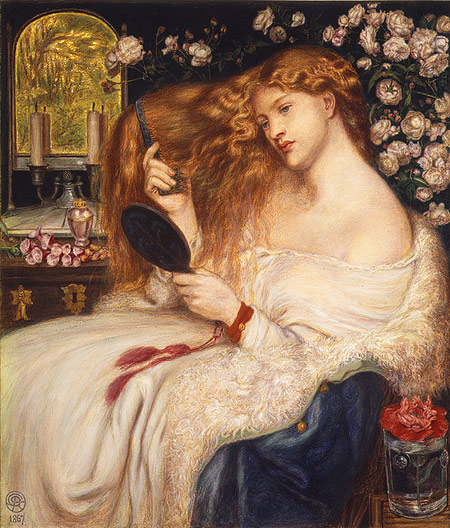
\includegraphics[width=0.40\textwidth]{Images/Rossetti_lady_lilith_1867}
	\\ {\small Rosetti 1867, Lady Lilith.}
\end{wrapfigure}


She, like Susan, was human once. She was the first woman. You see, women did not actually come from Adams rib. At least not the first. Lilith and Adam were both created from the dust to be each others companion. Adam preferred for her to be obedient to him and she preferred to have an equal partner and when that didn't work out she left. God only knows where she went but along the way she met Sam\ae l and they have been inseparable ever since.

She is the worlds first polyamorous woman. Sam\ae l may be her primary so to speak but she has had many lovers. Unlike the accusations of her being a whore though she genuinely loves those she is with and is quite happy, her and Sam\ae l are still together so they are an example of a successful polyamorous relationship.

She is a fierce advocate of women's sexuality, she enjoys sex with both men and women(not physically I assume, she's a d\ae mon), so as a result is an LGBT advocate. I'm sure that she is a 3rd generation feminist. She protects pregnant women and children. She is a healer. Although she heals through the feminine current she heals both men and women, especially with self image.

She is drop dead gorgeous. Everyone who sees her sees her differently but the description I was given makes her sound like an irish sex god. Long wavy red hair, pale skin and red lips, deep emerald green eyes, perfect body. She either wears nothing or majestic see through clothing.

What I have said I have said. There is such a conflicting mess in the field of demonology. Lilith likely has a dozen names at least. Her three most popular are Lilith, Lamia and Lamashtu. Sure they could be different entities but Lamashtu for one was described as being the daughter of heaven. In the context given it meant that God created her from nothing, as opposed to coming from man or woman. That has to be Lilith. 

Why is Lilith often described as evil incarnate? Sexually liberated feminist women and LGBT people are discriminated against now, whether they were Gods or not how would people have treated them or spoken of them in 1000BC or even before? People are so quick to see monsters around them, if only they would spend that time looking for the monsters inside themselves.
\chapter{Legal Licence}
The media source is available at \textit{https://eteepell.github.io/Susans-Requiem} under the following license.\\

Creative Commons Attribution-ShareAlike 4.0 International Public License

By exercising the Licensed Rights (defined below), You accept and agree to be bound by the terms and conditions of this Creative Commons Attribution-ShareAlike 4.0 International Public License ("Public License"). To the extent this Public License may be interpreted as a contract, You are granted the Licensed Rights in consideration of Your acceptance of these terms and conditions, and the Licensor grants You such rights in consideration of benefits the Licensor receives from making the Licensed Material available under these terms and conditions.

Section 1 – Definitions.

    Adapted Material means material subject to Copyright and Similar Rights that is derived from or based upon the Licensed Material and in which the Licensed Material is translated, altered, arranged, transformed, or otherwise modified in a manner requiring permission under the Copyright and Similar Rights held by the Licensor. For purposes of this Public License, where the Licensed Material is a musical work, performance, or sound recording, Adapted Material is always produced where the Licensed Material is synched in timed relation with a moving image.
    Adapter's License means the license You apply to Your Copyright and Similar Rights in Your contributions to Adapted Material in accordance with the terms and conditions of this Public License.
    BY-SA Compatible License means a license listed at creativecommons.org/compatiblelicenses, approved by Creative Commons as essentially the equivalent of this Public License.
    Copyright and Similar Rights means copyright and/or similar rights closely related to copyright including, without limitation, performance, broadcast, sound recording, and Sui Generis Database Rights, without regard to how the rights are labeled or categorized. For purposes of this Public License, the rights specified in Section 2(b)(1)-(2) are not Copyright and Similar Rights.
    Effective Technological Measures means those measures that, in the absence of proper authority, may not be circumvented under laws fulfilling obligations under Article 11 of the WIPO Copyright Treaty adopted on December 20, 1996, and/or similar international agreements.
    Exceptions and Limitations means fair use, fair dealing, and/or any other exception or limitation to Copyright and Similar Rights that applies to Your use of the Licensed Material.
    License Elements means the license attributes listed in the name of a Creative Commons Public License. The License Elements of this Public License are Attribution and ShareAlike.
    Licensed Material means the artistic or literary work, database, or other material to which the Licensor applied this Public License.
    Licensed Rights means the rights granted to You subject to the terms and conditions of this Public License, which are limited to all Copyright and Similar Rights that apply to Your use of the Licensed Material and that the Licensor has authority to license.
    Licensor means the individual(s) or entity(ies) granting rights under this Public License.
    Share means to provide material to the public by any means or process that requires permission under the Licensed Rights, such as reproduction, public display, public performance, distribution, dissemination, communication, or importation, and to make material available to the public including in ways that members of the public may access the material from a place and at a time individually chosen by them.
    Sui Generis Database Rights means rights other than copyright resulting from Directive 96/9/EC of the European Parliament and of the Council of 11 March 1996 on the legal protection of databases, as amended and/or succeeded, as well as other essentially equivalent rights anywhere in the world.
    You means the individual or entity exercising the Licensed Rights under this Public License. Your has a corresponding meaning.

Section 2 – Scope.

    License grant.
        Subject to the terms and conditions of this Public License, the Licensor hereby grants You a worldwide, royalty-free, non-sublicensable, non-exclusive, irrevocable license to exercise the Licensed Rights in the Licensed Material to:
            reproduce and Share the Licensed Material, in whole or in part; and
            produce, reproduce, and Share Adapted Material.
        Exceptions and Limitations. For the avoidance of doubt, where Exceptions and Limitations apply to Your use, this Public License does not apply, and You do not need to comply with its terms and conditions.
        Term. The term of this Public License is specified in Section 6(a).
        Media and formats; technical modifications allowed. The Licensor authorizes You to exercise the Licensed Rights in all media and formats whether now known or hereafter created, and to make technical modifications necessary to do so. The Licensor waives and/or agrees not to assert any right or authority to forbid You from making technical modifications necessary to exercise the Licensed Rights, including technical modifications necessary to circumvent Effective Technological Measures. For purposes of this Public License, simply making modifications authorized by this Section 2(a)(4) never produces Adapted Material.
        Downstream recipients.
            Offer from the Licensor – Licensed Material. Every recipient of the Licensed Material automatically receives an offer from the Licensor to exercise the Licensed Rights under the terms and conditions of this Public License.
            Additional offer from the Licensor – Adapted Material. Every recipient of Adapted Material from You automatically receives an offer from the Licensor to exercise the Licensed Rights in the Adapted Material under the conditions of the Adapter’s License You apply.
            No downstream restrictions. You may not offer or impose any additional or different terms or conditions on, or apply any Effective Technological Measures to, the Licensed Material if doing so restricts exercise of the Licensed Rights by any recipient of the Licensed Material.
        No endorsement. Nothing in this Public License constitutes or may be construed as permission to assert or imply that You are, or that Your use of the Licensed Material is, connected with, or sponsored, endorsed, or granted official status by, the Licensor or others designated to receive attribution as provided in Section 3(a)(1)(A)(i).

    Other rights.
        Moral rights, such as the right of integrity, are not licensed under this Public License, nor are publicity, privacy, and/or other similar personality rights; however, to the extent possible, the Licensor waives and/or agrees not to assert any such rights held by the Licensor to the limited extent necessary to allow You to exercise the Licensed Rights, but not otherwise.
        Patent and trademark rights are not licensed under this Public License.
        To the extent possible, the Licensor waives any right to collect royalties from You for the exercise of the Licensed Rights, whether directly or through a collecting society under any voluntary or waivable statutory or compulsory licensing scheme. In all other cases the Licensor expressly reserves any right to collect such royalties.

Section 3 – License Conditions.

Your exercise of the Licensed Rights is expressly made subject to the following conditions.

    Attribution.

        If You Share the Licensed Material (including in modified form), You must:
            retain the following if it is supplied by the Licensor with the Licensed Material:
                identification of the creator(s) of the Licensed Material and any others designated to receive attribution, in any reasonable manner requested by the Licensor (including by pseudonym if designated);
                a copyright notice;
                a notice that refers to this Public License;
                a notice that refers to the disclaimer of warranties;
                a URI or hyperlink to the Licensed Material to the extent reasonably practicable;
            indicate if You modified the Licensed Material and retain an indication of any previous modifications; and
            indicate the Licensed Material is licensed under this Public License, and include the text of, or the URI or hyperlink to, this Public License.
        You may satisfy the conditions in Section 3(a)(1) in any reasonable manner based on the medium, means, and context in which You Share the Licensed Material. For example, it may be reasonable to satisfy the conditions by providing a URI or hyperlink to a resource that includes the required information.
        If requested by the Licensor, You must remove any of the information required by Section 3(a)(1)(A) to the extent reasonably practicable.
    ShareAlike.

    In addition to the conditions in Section 3(a), if You Share Adapted Material You produce, the following conditions also apply.
        The Adapter’s License You apply must be a Creative Commons license with the same License Elements, this version or later, or a BY-SA Compatible License.
        You must include the text of, or the URI or hyperlink to, the Adapter's License You apply. You may satisfy this condition in any reasonable manner based on the medium, means, and context in which You Share Adapted Material.
        You may not offer or impose any additional or different terms or conditions on, or apply any Effective Technological Measures to, Adapted Material that restrict exercise of the rights granted under the Adapter's License You apply.

Section 4 – Sui Generis Database Rights.

Where the Licensed Rights include Sui Generis Database Rights that apply to Your use of the Licensed Material:

    for the avoidance of doubt, Section 2(a)(1) grants You the right to extract, reuse, reproduce, and Share all or a substantial portion of the contents of the database;
    if You include all or a substantial portion of the database contents in a database in which You have Sui Generis Database Rights, then the database in which You have Sui Generis Database Rights (but not its individual contents) is Adapted Material, including for purposes of Section 3(b); and
    You must comply with the conditions in Section 3(a) if You Share all or a substantial portion of the contents of the database.

For the avoidance of doubt, this Section 4 supplements and does not replace Your obligations under this Public License where the Licensed Rights include other Copyright and Similar Rights.

Section 5 – Disclaimer of Warranties and Limitation of Liability.

    Unless otherwise separately undertaken by the Licensor, to the extent possible, the Licensor offers the Licensed Material as-is and as-available, and makes no representations or warranties of any kind concerning the Licensed Material, whether express, implied, statutory, or other. This includes, without limitation, warranties of title, merchantability, fitness for a particular purpose, non-infringement, absence of latent or other defects, accuracy, or the presence or absence of errors, whether or not known or discoverable. Where disclaimers of warranties are not allowed in full or in part, this disclaimer may not apply to You.
    To the extent possible, in no event will the Licensor be liable to You on any legal theory (including, without limitation, negligence) or otherwise for any direct, special, indirect, incidental, consequential, punitive, exemplary, or other losses, costs, expenses, or damages arising out of this Public License or use of the Licensed Material, even if the Licensor has been advised of the possibility of such losses, costs, expenses, or damages. Where a limitation of liability is not allowed in full or in part, this limitation may not apply to You.

    The disclaimer of warranties and limitation of liability provided above shall be interpreted in a manner that, to the extent possible, most closely approximates an absolute disclaimer and waiver of all liability.

Section 6 – Term and Termination.

    This Public License applies for the term of the Copyright and Similar Rights licensed here. However, if You fail to comply with this Public License, then Your rights under this Public License terminate automatically.

    Where Your right to use the Licensed Material has terminated under Section 6(a), it reinstates:
        automatically as of the date the violation is cured, provided it is cured within 30 days of Your discovery of the violation; or
        upon express reinstatement by the Licensor.
    For the avoidance of doubt, this Section 6(b) does not affect any right the Licensor may have to seek remedies for Your violations of this Public License.
    For the avoidance of doubt, the Licensor may also offer the Licensed Material under separate terms or conditions or stop distributing the Licensed Material at any time; however, doing so will not terminate this Public License.
    Sections 1, 5, 6, 7, and 8 survive termination of this Public License.

Section 7 – Other Terms and Conditions.

    The Licensor shall not be bound by any additional or different terms or conditions communicated by You unless expressly agreed.
    Any arrangements, understandings, or agreements regarding the Licensed Material not stated herein are separate from and independent of the terms and conditions of this Public License.

Section 8 – Interpretation.

    For the avoidance of doubt, this Public License does not, and shall not be interpreted to, reduce, limit, restrict, or impose conditions on any use of the Licensed Material that could lawfully be made without permission under this Public License.
    To the extent possible, if any provision of this Public License is deemed unenforceable, it shall be automatically reformed to the minimum extent necessary to make it enforceable. If the provision cannot be reformed, it shall be severed from this Public License without affecting the enforceability of the remaining terms and conditions.
    No term or condition of this Public License will be waived and no failure to comply consented to unless expressly agreed to by the Licensor.
    Nothing in this Public License constitutes or may be interpreted as a limitation upon, or waiver of, any privileges and immunities that apply to the Licensor or You, including from the legal processes of any jurisdiction or authority.

Creative Commons is not a party to its public licenses. Notwithstanding, Creative Commons may elect to apply one of its public licenses to material it publishes and in those instances will be considered the “Licensor.” The text of the Creative Commons public licenses is dedicated to the public domain under the CC0 Public Domain Dedication. Except for the limited purpose of indicating that material is shared under a Creative Commons public license or as otherwise permitted by the Creative Commons policies published at creativecommons.org/policies, Creative Commons does not authorize the use of the trademark “Creative Commons” or any other trademark or logo of Creative Commons without its prior written consent including, without limitation, in connection with any unauthorized modifications to any of its public licenses or any other arrangements, understandings, or agreements concerning use of licensed material. For the avoidance of doubt, this paragraph does not form part of the public licenses.

Creative Commons may be contacted at creativecommons.org.



% begin back matter

\end{document}
% END THE DOCUMENT


